\documentclass[a4paper]{scrreprt}

\usepackage[german]{babel}
\usepackage[utf8]{inputenc}
\usepackage[T1]{fontenc}
\usepackage{ae}
\usepackage[bookmarks,bookmarksnumbered]{hyperref}
\usepackage{graphicx}
\usepackage[toc]{glossaries}
\usepackage{float}
\graphicspath{ {Images/} }
\setcounter{secnumdepth}{5}
\makeglossaries

\begin{document}
    \newglossaryentry{Studienleiter}{name=Studienleiter, description={Person, unter dessen Leitung eine Studie durchgeführt wird}}
    \newglossaryentry{Proband}{name=Proband, description={Leute, der sich an einer Studie beteiligt}}
    \newglossaryentry{Web-Interface}{name=Web-Interface, description={Benutzeroberfläche, die man in einem Web-Browser nutzen kann}}
    \newglossaryentry{Antwortsstatus}{name=Antwortsstatus, description={Die statistischen Daten der Antworten von Probanden innerhalb von G\"ultigkeitszeitbereich des Fragebogens}}
    \newglossaryentry{Android-App}{name=Android-App, description={Anwendungssoftware für Mobilgeräte mit Android als Betriebssystem}}
    %\newglossaryentry{Aussch\"opfungsquote}{name=Aussch\"opfungsquote, description={der Quotient aus die Anzahl der Probanden, die eine Frage tatsächlich beantworteten und die Anzahl aller Probanden (Die Ausschöpfungsquoten sind also global und für alle Probanden gleich.)}}

    \begin{flushright}
        
\includegraphics[scale = 0.7]{kit-logo.jpg}\\[0.5cm]
        % 
\includegraphics[scale = 1]{teco.jpg}
    \end{flushright}
    % 
\includegraphics[scale = 0.5]{kit-logo.jpg} \hspace{4cm} 
\includegraphics[scale = 1]{teco.jpg}
    \vspace*{2cm}

    \begin{center} \large

        Praxis der Softwareentwicklung
        \vspace * {1.5cm}

        \textbf{\huge Mind Rate}

        \vspace*{1cm}


        {\Large Ein interaktives System mit Android-Client f\"ur Studien nach Experience-Sampling-Method (ESM)}

        \vspace*{1cm}

        \textbf{\Large Pflichtenheft}
        \vspace*{2cm}

        Shanshan Du, Yi Ge, Renhan Lou, Ruoheng Ma, Haobin Tan
        \vspace*{1cm}

        02. Dezember 2016
        \vspace*{2.5cm}

        Betreuung: Anja Exler, Dr. Andrea Schankin\\[0.5cm]
        Forschungsgruppe TECO: Technology for Pervasive Computing\\[0.5cm]

        Karlsruher Institut für Technologie
    \end{center}
    \thispagestyle{empty}

    \tableofcontents

    \chapter{Zielbestimmung}

        \noindent Das Produkt besteht aus zwei Teilsysteme: ein \gls{Web-Interface} für den \gls{Studienleiter} und eine \gls{Android-App} für die \gls{Proband}en. Der \gls{Studienleiter} soll durch das Produkt in die Lage versetzt werden, Studien nach ESM durchzuf\"uhren. Die Probanden k\"onnen sich an den Studien beteiligen, wobei sie die \gls{Android-App} nutzen.


        \section{Musskriterien}
            \subsection{\gls{Web-Interface} für \gls{Studienleiter}}

                \subsubsection{Verwalten der Studien}
                    \begin{itemize}
                        \item Erfassen von Pers\"onlichen Daten der Probanden (Alter, Geschlecht, Beruf)
                        % \item Erstellen, \"Andern von Studien
                        \item Setzen von Namen, ID und Dauer der Studien
                    \end{itemize}

                \subsubsection{Verwalten der Frageb\"ogen}
                    \begin{itemize}
                        \item Erstellen, Ändern von Fragebögen
                        \item Erstellen, \"Andern von Fragen verschiedener Typen
                        \item Setzen, \"Andern von auslösenden Ereiginissen und Abgabeterminen der Frageb\"ogen
                    \end{itemize}

                \subsubsection{Erfassen von Ergebnisse der Untersuchung}
                    \begin{itemize}
                        \item Besichtigen von \gls{Antwortsstatus}
                        \item Exportieren von Daten in CSV-Format
                    \end{itemize}
            \vspace*{0.5cm}

            \subsection{\gls{Android-App} f\"ur \gls{Proband}en}

                \subsubsection{Anmelden mit Studie-ID}
                    \begin{itemize}
                        \item Eingeben von Studie-ID
                        \item Eingeben von Alter, Geschlecht, Beruf des Probanden
                    \end{itemize}

                \subsubsection{Antwort auf Frageb\"ogen}
                    \begin{itemize}
                        \item Notifikationen über die Fragebögen
                        \item Beantworten von Frageb\"ogen
                    \end{itemize}

                \subsubsection{Auslösen von Fragebögen durch verschiedene Ereignisse}
                    \begin{itemize}
                        \item Motion-Sensor (Beschleunigung, Gravitation, Rotation)
                        \item Environmental-Sensor (Temperatur, Licht, Luftdruck, relative Luftfeuchtigkeit)
                        \item Positon-Sensor (Richtung, Magnetfeld, Nähe)
                        \item Zeit
                        \item Kalender
                        \item Notifikationen von anderen Apps
                        \item Ereignisdaten werden gespeichert und mit den Antworten zusammen hochgeladen
                    \end{itemize}

                \subsubsection{Automatische Verwaltung von Antworten}
                    \begin{itemize}
                        \item lokales Speichern von Antworten
                        \item Protokollieren von Abgabezeit der Antworten
                        \item Hochladen von Antworten (inkl. der protokollierten Ereignisdaten) auf den Server
                    \end{itemize}


                \vspace*{0.5cm}


        \section{Wunschkriterien}

            \subsection{\gls{Web-Interface} f\"ur \gls{Studienleiter}}
                \begin{itemize}
                    \item Senden von Nachrichten zu allen \gls{Proband}en einer Studie
                    \item Erm\"oglichen von ``angemeldet bleiben"
                    \item Erzeugen von verschiedenen (Statistik-)Diagramme f\"ur hochgeladene Daten (z.B. S\"aulendiagramm, Kreisdiagramm)
                    \item Unterst\"utzen von unterschiedlichen Sprachen
                    \item Setzen von Zeitabstand zwischen 2 Frageb\"ogen

                \end{itemize}

            \subsection{Android-Anwendung f\"ur \gls{Proband}en}
                \begin{itemize}
                    \item Erm\"oglichen von ``angemeldet bleiben"
                    \item Unterst\"utzen von unterschiedlichen Sprachen
                \end{itemize}
                \vspace*{0.5cm}


        \section{Abgrenzungskriterien}
            % Abgrenzungskriterien: Diese Kriterien sollen bewusst nicht erreicht werden.
            \begin{itemize}
                \item Keine verteilte Datenbank, keine Echtzeitanforderungen, keine synchronisierten Datenbankzugriffe
                \item Keine Unterst\"utzung f\"ur iOS
            \end{itemize}

    \chapter{Produkteinsatz}
        Das Produkt dient zur Sammlung der Studiendaten aus ESM-Studien. Damit bietet sie für \gls{Studienleiter} eine Lösung, ESM-Studien durchzuführen. Diese Tätigkeit soll zusätzlich im Internet und auf dem Smartphone möglich sein.

        \section{Anwendungsbereiche}
            \begin{itemize}
                \item Akademischer / Sozialwissenschaftlicher Anwendungsbereich
                \item Statistischer Anwendungsbereich
                \item Geschäftlicher Anwendungsbereich
            \end{itemize}

        \section{Zielgruppen}
            \begin{itemize}
                \item \gls{Studienleiter} einer ESM-Studie
                \item Teilnehmer der Studie
            \end{itemize}

        \section{Betriebsbedingungen}
            \begin{itemize}
                \item \gls{Studienleiter}: Büroumgebung
                \item Studienteilnehmer: im alltäglichen Leben aufs Smartphone
                \item Betriebszeit rund um die Uhr, läuft unbeaufsichtigt
            \end{itemize}

    \chapter{Produktumgebung}
        Eine Client-Server Architektur mit 2 Client-Typen: ein \gls{Web-Interface} für \gls{Studienleiter} und eine \gls{Android-App} für \gls{Proband}en

        \section{Software}
            \begin{itemize}
                \item Serverseite
                    \begin{itemize}
                        \item  Läuft auf Linux
                        \item Alle Softwares der Serverseite werden durch Docker verpackt
                        \item Datenbank: SQLite, verwaltet durch das Django-Framework
                        \item Programmiersprache: Python 3
                        \item Web server: Nginx
                    \end{itemize}
                \item Clientseite
                    \begin{itemize}
                        \item \gls{Web-Interface}\\
                             Web-Browser, Referenzstandard Google Chrome 54
                        \item  \gls{Android-App}\\
                             Android, Referenzstandard Android 5.1.1 Lollipop
                    \end{itemize}
            \end{itemize}

        \section{Hardware}
            \begin{itemize}
                \item Serverseite\\
                    Leistungsstarke Standardrechner
                \item  \gls{Web-Interface}\\
                    Standardrechner (für Web-Browser)
                \item \gls{Android-App}\\
                    Standardsmartphone
            \end{itemize}

    \chapter{Funktionale Anforderungen}

        \section{\gls{Web-Interface}}
            \begin{itemize}
                \item \textbf{/F10/ Registrieren und Anmelden der \gls{Studienleiter}}

                    \par \textbf{Ziel: }Registrieren oder Anmelden der \gls{Studienleiter} in der Web-Verwaltungssystem
                    \par \textbf{Vorbedingung (Registrieren): }-keine-
                    \par \textbf{Vorbedingung (Anmelden): }Ein Konto des Leiters soll vorhanden sein.
                    \par \textbf{Nachbedingung (erfolgreiches Registrieren): }Der Leiter bekommt eine Bestätigungsmail und kann sich mit dem neu erzeugten Konto anmelden.
                    \par \textbf{Nachbedingung (erfolgreiches Anmelden): }Der Leiter ist in der Verwaltungssystem angemeldet und kann seine Studien verwalten.
                    \par \textbf{Nachbedingung (Fehlschlag): }Der Leiter bleibt unangemeldet.
                    \par \textbf{Akteure: }\gls{Studienleiter}
                    \par \textbf{Auslösendes Ereignis: }Der Leiter busucht die Webseite dieses Online-Verwaltungssystems.
                    \par \textbf{Beschreibung: }
                        \begin{enumerate}
                            \item Beim Registrieren soll der Leiter eine gültige Email-Adresse als Konto-Name und ein gültiges Passwort eintragen. Diese Daten werden von dem Datenbank gespeichert und der Server erzeugt ein neues Konto. Danach empfängt der Leiter eine Bestätigungsmail und kann sich mit dem neuen Konto anmelden.
                            \item Beim Anmelden soll der Leiter die registrierte Email-Adresse und sein Passwort eingeben. Wenn die Email-Adresse und das Passwort stimmen überein, dann wird der Leiter in die Verwaltungsseite weitergeleitet.
                        \end{enumerate}
                    \par \textbf{Erweiterung: }
                    \par \textbf{Alternativen: }


                \item \textbf{/F20/ Vergessendes Passwort neu setzen}

                \par \textbf{Ziel: }\gls{Studienleiter} können vergessendes Passwort neu setzen
                \par \textbf{Vorbedingung: }\gls{Studienleiter} hat ein Konto
                \par \textbf{Nachbedingung (Konto vorhanden): }Der \gls{Studienleiter} bekommt ein neues zufällig generiertes Passwort.
                \par \textbf{Nachbedingung (Konto nicht vorhanden): }Eine Fehlermeldung mit den Wörtern ``Account does not exist'' erscheint.
                \par \textbf{Akteure: }\gls{Studienleiter}
                \par \textbf{Auslösendes Ereignis: }Der \gls{Studienleiter} klickt auf ``Reset Password''
                \par \textbf{Beschreibung: }
                \begin{enumerate}
                    \item Auf ``Reset Password'' klicken
                    \item Email-Adresse eingeben
                    \item Der \gls{Studienleiter} bekommt ein Mail mit einem neuen zufällig generierten Passwort
                \end{enumerate}
                \par \textbf{Erweiterung: }
                    \par Falls das Konto nicht vorhanden ist, kommt eine Fehleranzeige sofort auf diese Seite auf. Sonst sendet der Server das Mail mit dem neuen Passwort zur Mailadresse des Kontos.


                \item \textbf{/F30/ Verwaltung des Fragebogens}

                \par \textbf{Ziel: }Verwaltung des Fragebogens in einer Studie
                \par \textbf{Vorbedingung: }Angemeldet in dem Verwaltungssystem und mindestens eine Studie vorhanden
                \par \textbf{Nachbedingung (Erfolg): }Ein neuer Fragebogen wird erstellt, oder ein vorliegender Fragebogen wird wieder eingestellt.
                \par \textbf{Nachbedingung (Fehlschlag): }Ein neuer Fragebogen wird nicht erstellt, oder ein vorliegender Fragebogen hat keine Änderung.
                \par \textbf{Akteure: }\gls{Studienleiter}
                \par \textbf{Auslösendes Ereignis: }Der \gls{Studienleiter} vesucht, den ``Set questionnaire'' Button auf der Webseite zu klicken

                \par \textbf{Beschreibung: }
                \begin{enumerate}
                    \item Wenn ein benötigter Fragebogen vorhanden ist, wählt der \gls{Studienleiter} diesen Fragebogen aus.
                    \item Wenn ein benötigter Fragebogen nicht vorhanden ist, klickt der \gls{Studienleiter} auf den Button ``new''
                    \item Der \gls{Studienleiter} gibt konkrete Name des Fragebogens ein
                    \item Der \gls{Studienleiter} stellt die Anfangsbedingungen des Fragebogens ein. Z.B. die Anfangszeit und die Endeszeit. Er kann auch die benötigte Sensoren hinzufügen.
                    \item Danach liegt eine Voransicht des Fragebogens rechts auf der Webseite vor
                    \item  Der \gls{Studienleiter} klickt auf den Button ``Refresh'', damit dir Inhalt des Fragebogens in den Voransicht gezeigt werden können
                    \item Der \gls{Studienleiter} klickt auf den Button ``save'', damit der Fragebogen in eine Studie gespeichert werden können
                    \item Der \gls{Studienleiter} klickt auf den Button ``submit'', damit der Fragebogen auf den Server hochgeladen werden können
                \end{enumerate}
                \par \textbf{Erweiterung: }
                \par \textbf{Alternativen: }
                \begin{figure}[H]
                    % \raggedleft
                    \centering
                    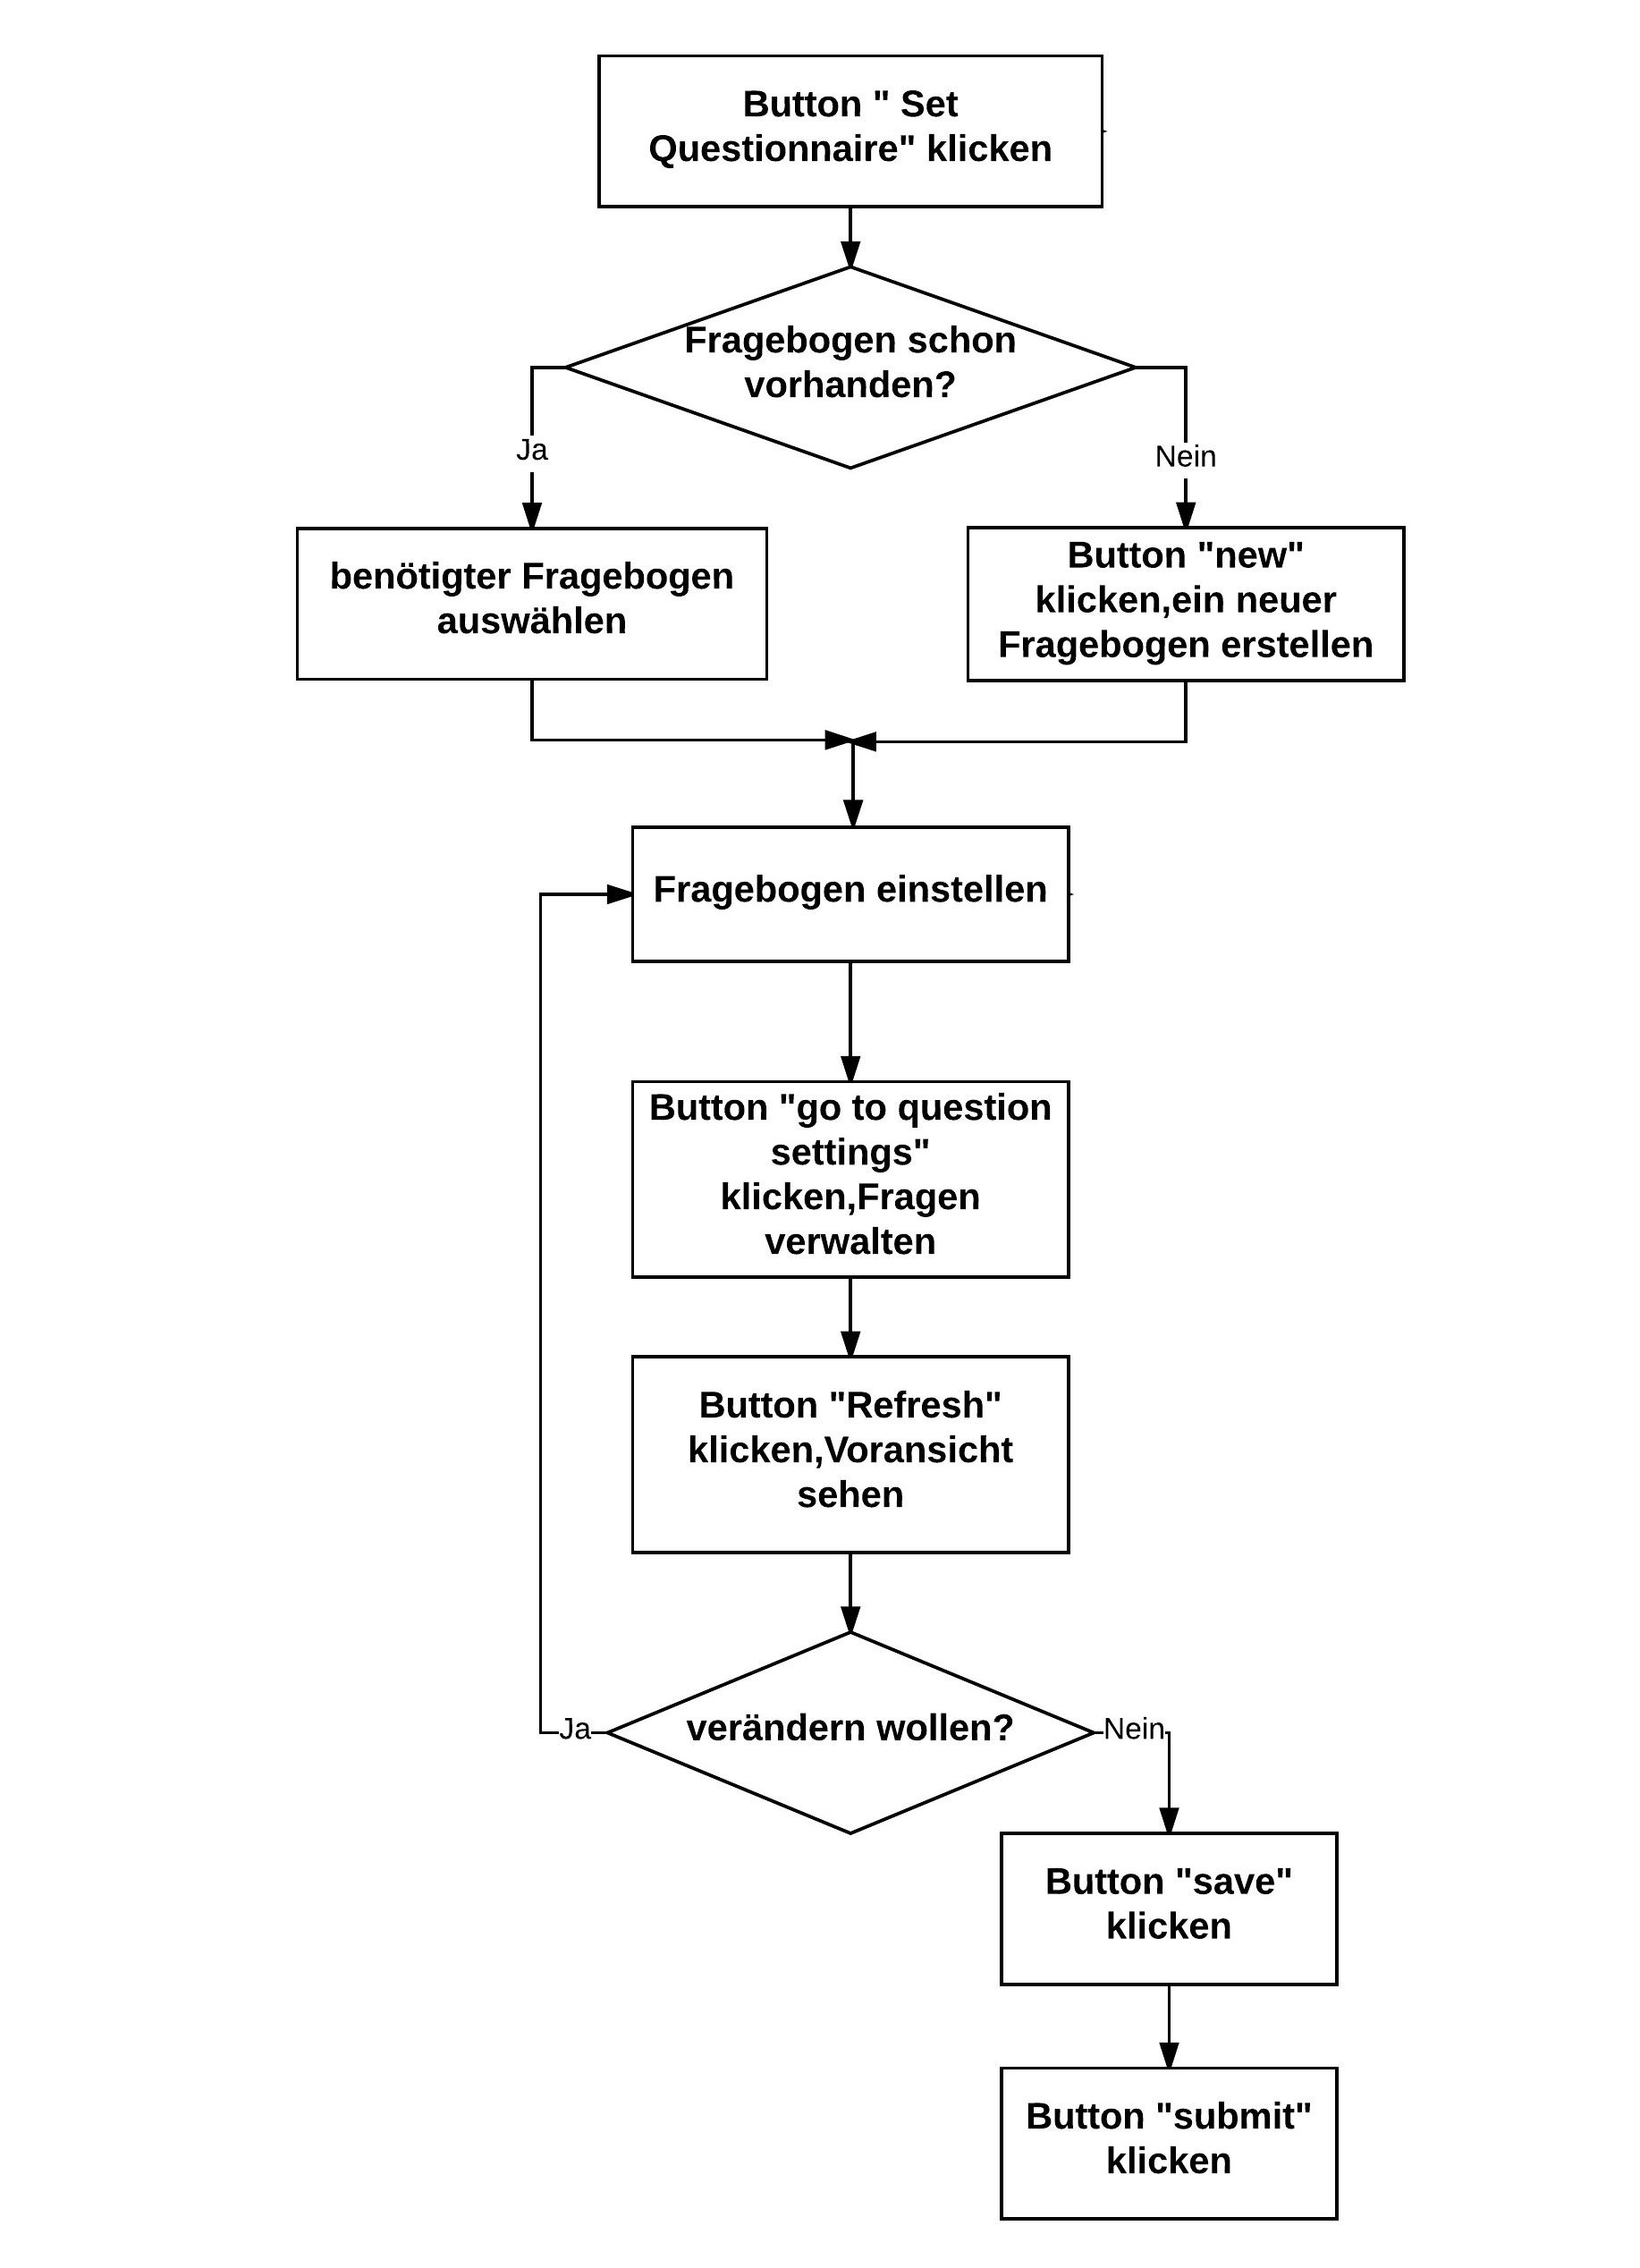
\includegraphics[scale=0.75]{FragebogenVerwaltung.jpeg}
                    \caption{Verwaltung des Fragebogen}
                \end{figure}


                \newpage

                \item \textbf{/F35/ Wählen von verschiedenen Erscheinungsereignissen der Fragebögen}
                
                \par \textbf{Ziel: }Studienleiter können verschiedene Erscheinungsereignisse für Fragebögen einstellen.
                \par \textbf{Vorbedingung: }Angemeldet in dem Verwaltungssystem und mindestens eine Studie vorhanden
                \par \textbf{Nachbedingung (Erfolg): }Ein neuer Frageboden mit Erscheinungsereignissen wird erstellt, oder die Erscheinungsereignisse eines vorliegenden Fragebogens wird eingestellt.
                \par \textbf{Nachbedingung (Fehlschlag): }Ein neuer Fragebogen wird nicht erstellt, oder ein vorliegender Fragebogen hat keine Änderung.
                \par \textbf{Akteure: }\gls{Studienleiter}
                \par \textbf{Auslösendes Ereignis: }Der \gls{Studienleiter} klickt auf den ``Set trigger event'' Button
                
                \par \textbf{Beschreibung: }
                    \begin{enumerate}
                        \item Die mögliche Erscheinungsereignisse bestehen aus Sensorereignissen (Beschleunigung, Gravitation, Rotation, Temperatur, Licht, Luftdruck, relative Luftfeuchtigkeit, Richtung, Magnetfeld, Nähe), Zeit, Kalender und Notifikationen von anderen Apps.
                        \item Wenn ein Fragebogen beantwortet wird, werden die Ereignisdaten gespeichert und mit den Antworten zusammen hochgeladen.
                        \item Der \gls{Studienleiter} kann wählen, ob ein Ereignis bei ``genau", ``größer" oder ``kleiner" von bestimmten Sensordaten ausgelöst werden soll.
                        \item Der \gls{Studienleiter} kann eine maximale Anzahl von Auslösen eines Fragebogens pro Tag bestimmen.
                        \item Der \gls{Studienleiter} kann einen minimalen Zeitabstand zwischen zwei Ereignissen bestimmen.
                        \item  Der \gls{Studienleiter} kann wählen, ob ein Ereignis am Anfang oder Ende eines Kalender-Termins ausgelöst werden soll.
                        \item  Der \gls{Studienleiter} kann wählen, ob ein Ereignis direkt nach einer Natifikation von Anderen Apps ausgelöst werden soll.
                    \end{enumerate}
                
                
                \item \textbf{/F40/ Verwaltung der Fragen }
                \par \textbf{Ziel: }Erstellung der Fragen in einem Fragebogen
                \par \textbf{Vorbedingung: } Angemeldet in dem Verwaltungssystem und mindestens ein Fragebogen vorhanden
                \par \textbf{Nachbedingung (Erfolg): }Eine neue Frage wird erstellt.
                \par \textbf{Nachbedingung (Fehlschlag): }Eine neue Frage wird nicht erstellt
                \par \textbf{Akteure: }\gls{Studienleiter}
                \par \textbf{Auslösendes Ereignis: }Der \gls{Studienleiter} vesucht, den ``go to question settings'' Button auf der Webseite zu klicken
                \par \textbf{Beschreibung: }
                \begin{enumerate}
                    \item Verwaltung des Fragebogen
                    \par Der \gls{Studienleiter} wählt zuerst einen Fragebogen aus oder erstellt er einen neuen Fragebogen. Zudem gehört die neue Frage.
                    \item Erstellung und Löschen der Fragen
                    \par Der \gls{Studienleiter} entscheidet sich die Fragenart und Antwortart. Dann soll der \gls{Studienleiter} auch konkrete Frage eingeben.Er kann auch eine ausgewählte Frage von der Fragenliste löschen
                    \item Verwaltung der Beziehungen zwischen Fragen
                    \par Der \gls{Studienleiter} entscheidet sich, welche Option in diesen Frage ein auslösendes Ereignis vorliegender Fragen ist.Dann gibt er Fragennummer ein.
                    \item Voransicht
                    \par Der \gls{Studienleiter} klickt auf den Button ``Refresh'', damit die hinzugefügte Frage in den Fragebogen gezeigt werden können
                \end{enumerate}
                \par \textbf{Erweiterung: }
                \begin{enumerate}
                    \item Es gibt fünf Fragenarten. Die sind jeweils ``Single-Choice-Frage'', ``Multiple-Choice-Frage'', ``Skala mit Stufen Frage'', ``Skala ohne Stufe Frage'' und ``Offene Frage''.
                    \item Es ist nicht notwendig, die \gls{Proband}en den Fragebogen sequenziell zu antworten. Der \gls{Studienleiter} kann sich entscheiden, welche Fragen die \gls{Proband}en antworten müssen und welche Fragen ein auslösende Ereignis haben.
                \end{enumerate}
                \par \textbf{Alternativen: }
                \begin{figure}[H]
                    % \raggedleft
                    \centering
                    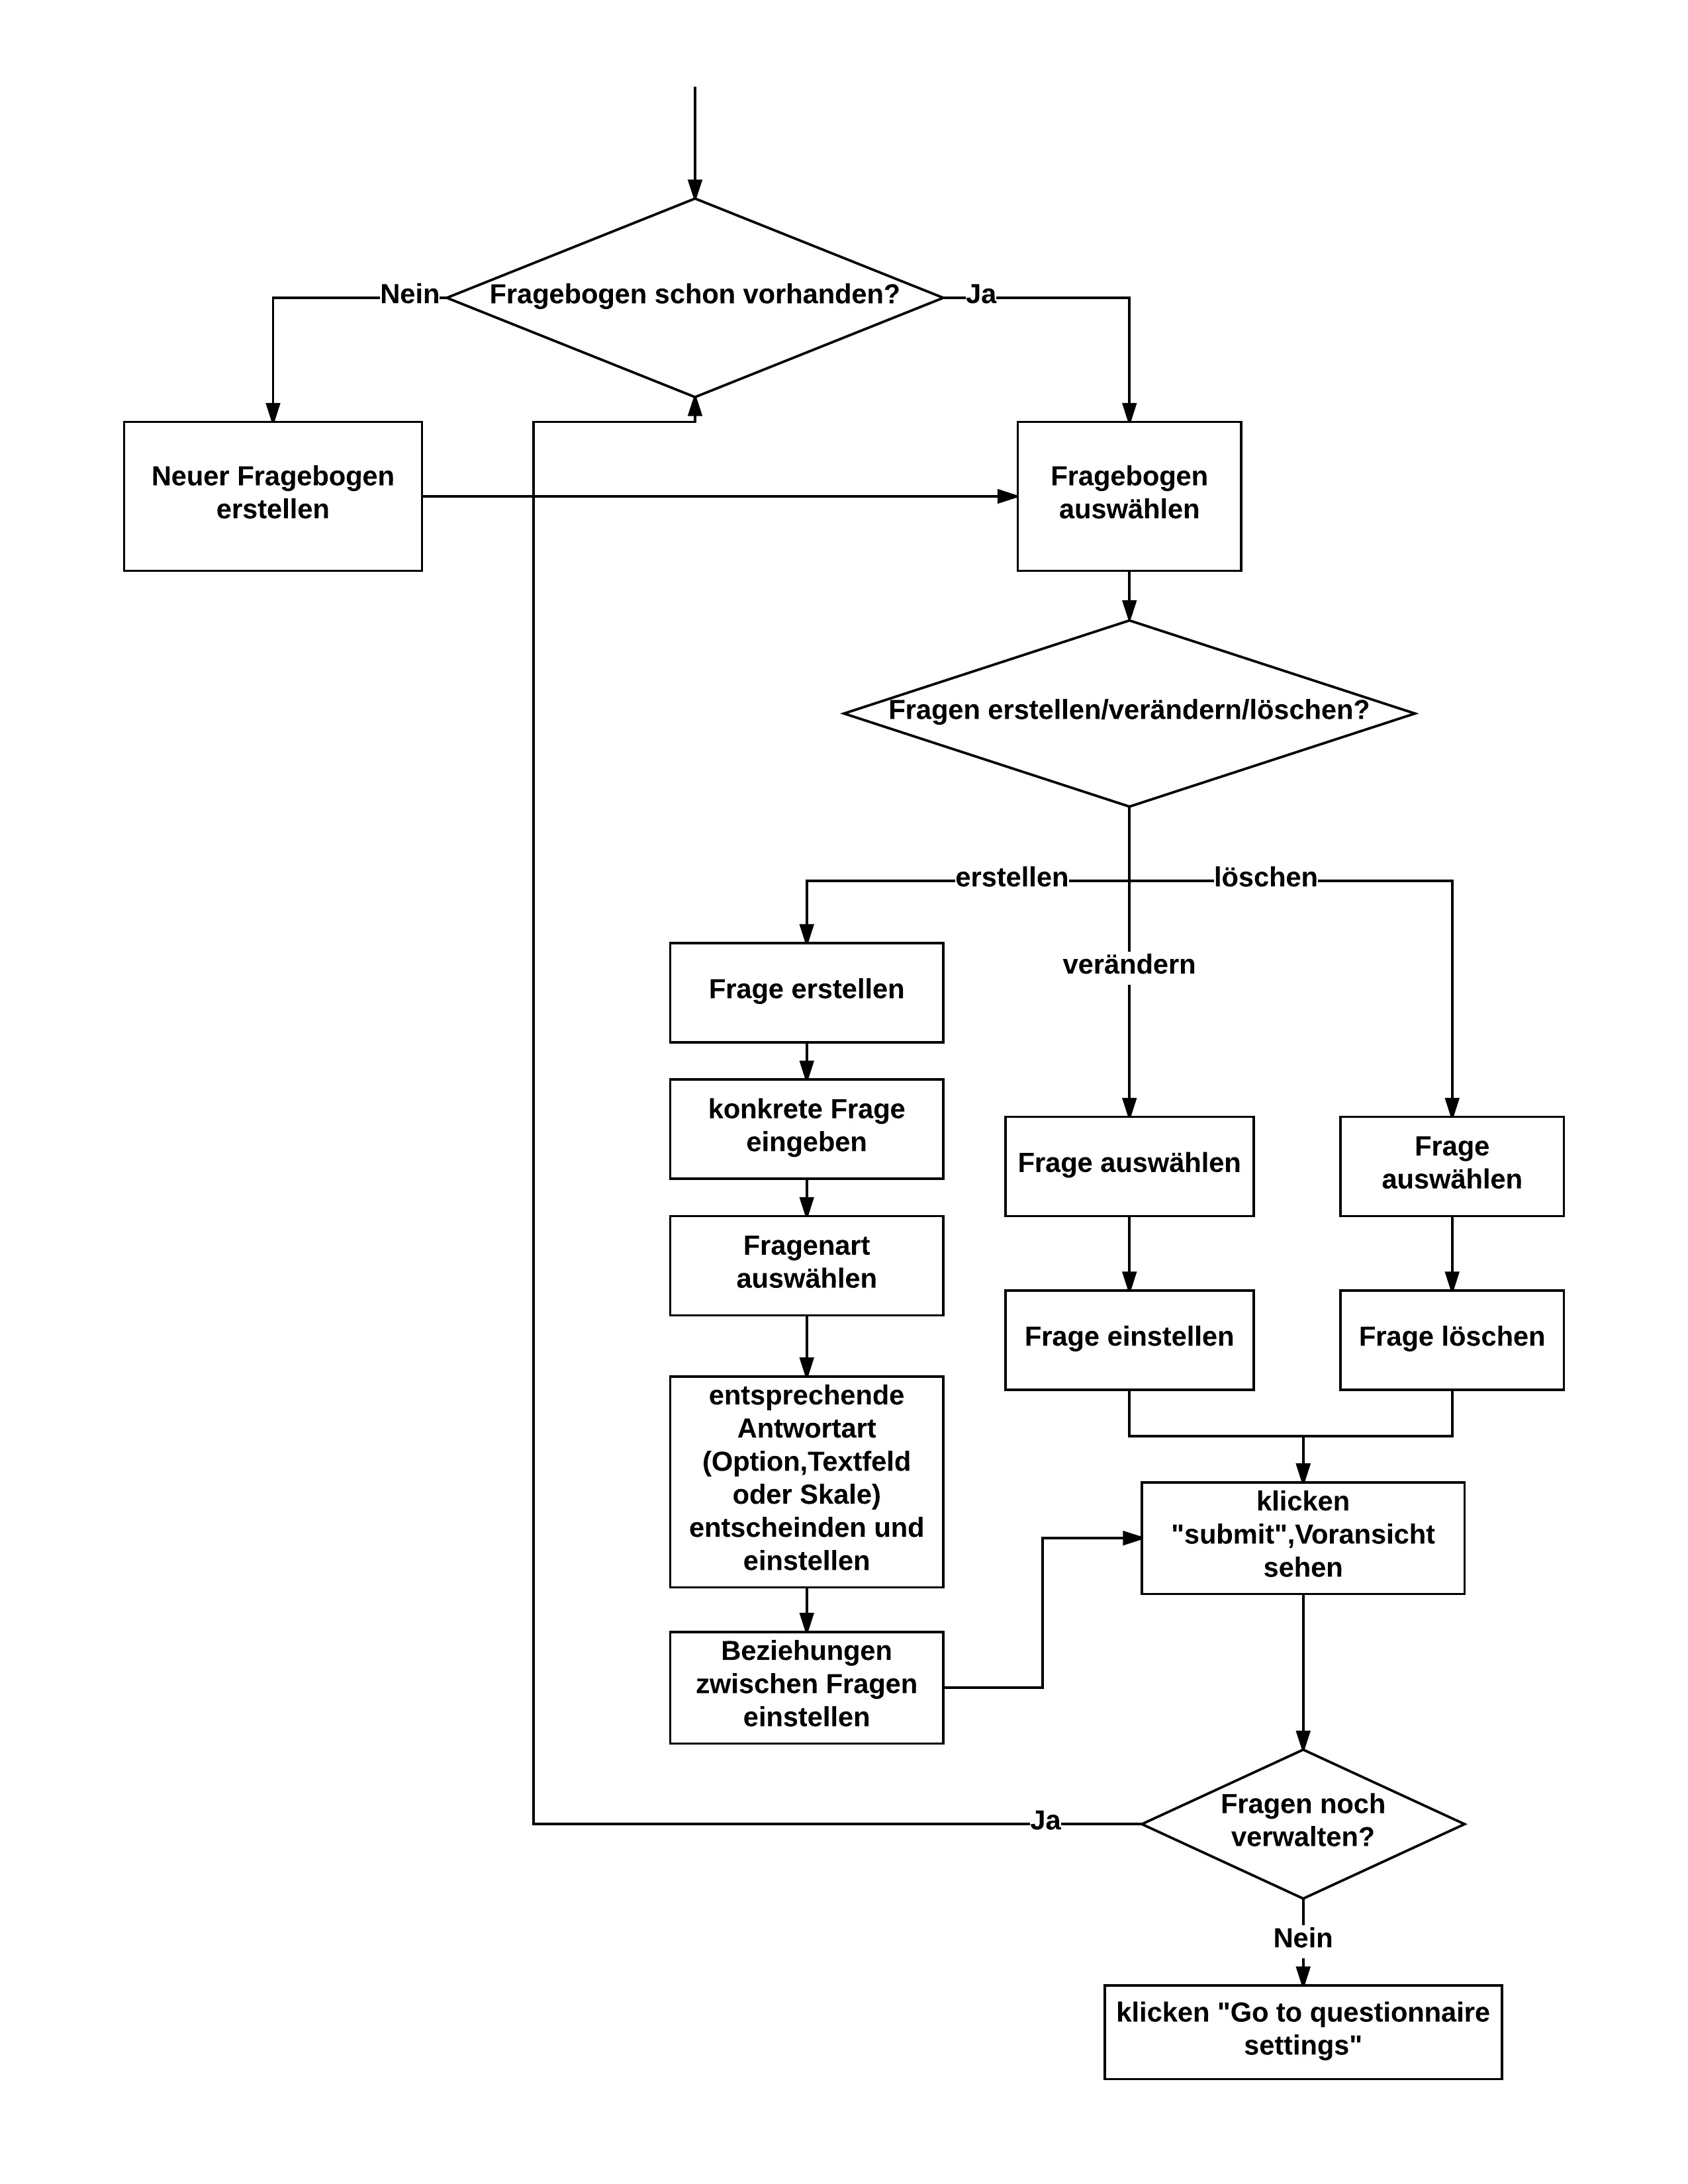
\includegraphics[scale=0.75]{FrageVerwaltung.jpeg}
                    \caption{Verwaltung der Fragen}
                \end{figure}

                \item \textbf{(Wunsch) /F50/ \gls{Antwortsstatus} besichtigen}
                \par \textbf{Ziel: }Besichtigung der Antwortsstatus
                \par \textbf{Vorbedingung: }Der \gls{Studienleiter} ist angemeldet.
                \par \textbf{Nachbedingung : }Der neue Antwortsstatus eines Fragebogens (z.B. Verteilung der Antwroten, Anzahl der beantworteten \gls{Proband}en) ist sichtbar.
                \par \textbf{Nachbedingung (Fehlschlag): }Der neue Antwortsstauts wird nicht gezeigt.
                \par \textbf{Akteure: }\gls{Studienleiter}
                \par \textbf{Auslösendes Ereignis: }Der \gls{Studienleiter} kann die \"Ubersicht von Antworten des aktuellen Fragebogens sehen.
                \par \textbf{Beschreibung: }
                \begin{enumerate}
                    \item Klicken von Button ``View answers''
                    \item Zeigen der \"Ubersicht von allen Antwort beim erfolgreichen Anmelden
                    % \item Erfassen von Antwortsstatus nach Bedarf und eingegebener Kriterien
                    \item Laden des neuen Antwortsstatus beim Klicken von Button ``Refresh''
                \end{enumerate}
                \par \textbf{Erweiterung: }
                \par \textbf{Alternativen: }
                \begin{figure}[H]
                    % \raggedleft
                    \centering
                    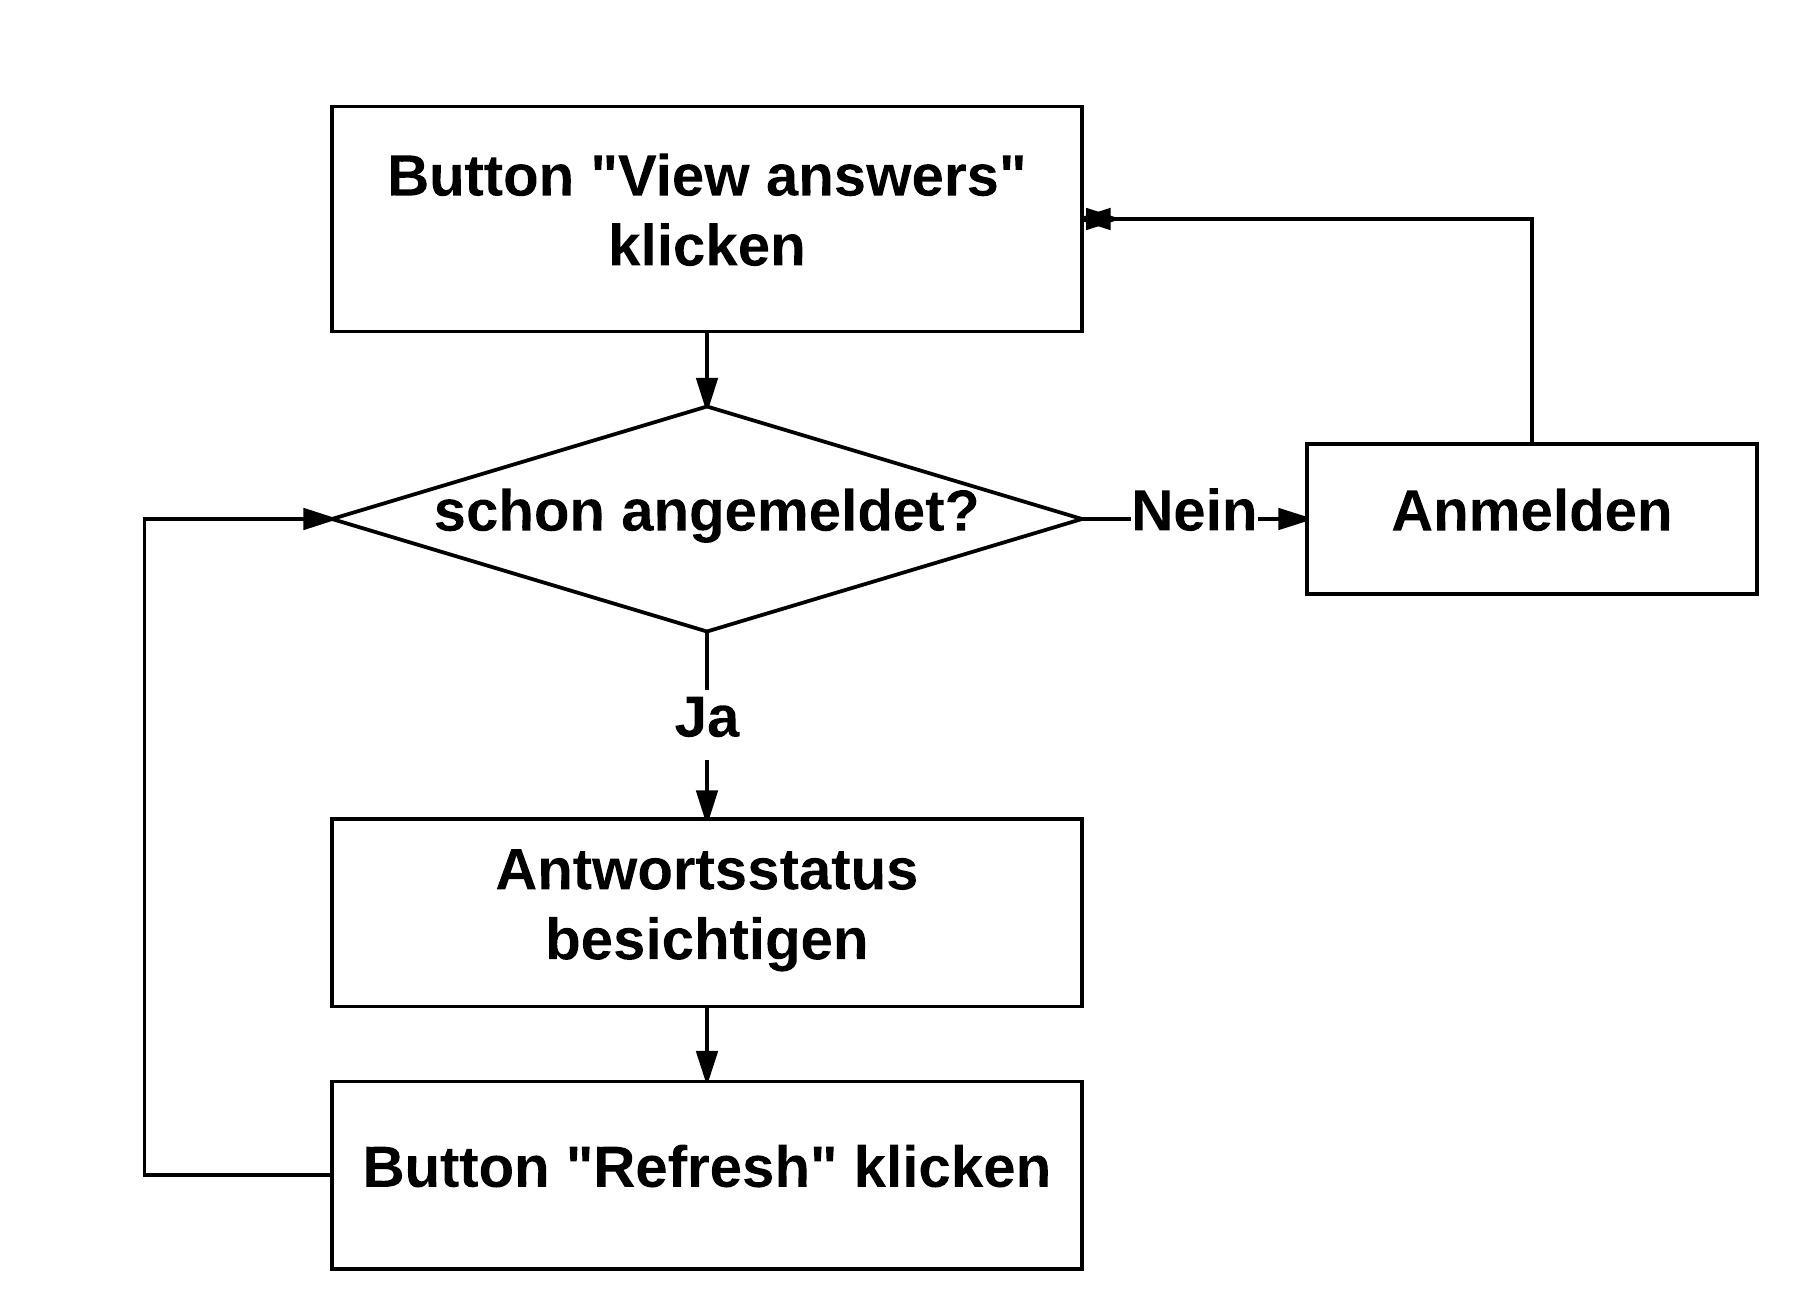
\includegraphics[scale=0.9]{Antwortsstatus_besichtigen.jpeg}
                    \caption{Antwortsstatus besichtigen}
                \end{figure}
                \newpage

                \item \textbf{(Wunsch) /F55/ Nachrichten zu allen \gls{Proband}en senden}
                \par \textbf{Ziel: }Senden von Nachrichten, um die \gls{Proband}en zu motivieren, die Fragebögen weiter zu beantworten.
                \par \textbf{Vorbedingung: }Der \gls{Studienleiter} ist angemeldet.
                \par \textbf{Nachbedingung : }Jeder \gls{Proband} erhalten Motivation vom \gls{Studienleiter}.
                \par \textbf{Nachbedingung (Fehlschlag): }Die \gls{Proband} erhalten keine Feedbacks.
                \par \textbf{Akteure: }\gls{Studienleiter}
                \par \textbf{Auslösendes Ereignis: }Alle \gls{Proband}en erhalten die von \gls{Studienleiter} geschriebene Motivation.
                \par \textbf{Beschreibung: }
                \begin{enumerate}
                    \item Klicken von Button ``Send Feedback / Motivation''
                    \item Schreiben von Feedback (Motivation)
                    \item Klicken von Button ``Send'', um die Feedbacks an allen \gls{Proband}en zu senden.
                \end{enumerate}
                \par \textbf{Erweiterung: }
                \par \textbf{Alternativen: }


                \item \textbf{/F60/Exportieren von Daten}

                \par \textbf{Ziel: }Exportieren von Antworten und statistischen Daten
                \par \textbf{Vorbedingung: }Angemeldet in dem Verwaltungssystem
                \par \textbf{Nachbedingung (Erfolg): }Die den Studien zugehörigen Daten werden in CSV-Format exportiert.
                \par \textbf{Nachbedingung (Fehlschlag): }Die den Studien zugehörigen Daten werden nicht exportiert.
                \par \textbf{Akteure: }\gls{Studienleiter}
                \par \textbf{Auslösendes Ereignis: }Der Leiter will die Daten exportieren.
                \par \textbf{Beschreibung: }
                \begin{itemize}
                    \item Der Leiter klickt auf ``Export data''. Dann werden die zugehörigen Daten in CSV-Format exportiert.
                \end{itemize}
            \end{itemize}


    \newpage
    \section{\gls{Android-App}}

        \begin{itemize}
            \item \textbf{/F70/Anmelden der \gls{Proband}en}

                \par \textbf{Ziel: }Anmelden der \gls{Proband}en in der App und Sammeln der Studienteilnehmerdaten bei dem ersten Anmelden
                \par \textbf{Vorbedingung: }-keine-
                \par \textbf{Nachbedingung (erstes Anmelden): }Studienteilnehmerdaten liegen vor und \gls{Proband} ist angemeldet
                \par \textbf{Nachbedingung (kein erstes Anmelden): }\gls{Proband} ist angemeldet
                \par \textbf{Akteure: }\gls{Proband}
                \par \textbf{Auslösendes Ereignis: }\gls{Proband} öffnet die App
                \par \textbf{Beschreibung: }
                \par 1. Wenn der \gls{Proband} zum ersten Mal die App öffnet: Der \gls{Proband} meldet sich mit der ID der Studie an und gibt die von \gls{Studienleiter} angeforderten Studienteilnehmerdaten ein. Eine einzigartige, mit dem Handy verbundene \gls{Proband}-ID wird generiert und dem \gls{Proband} zugeteilt. Die \gls{Proband}-ID wird nicht gezeigt aber in der App gespeichert. Die App wechselt dann auf die Hauptseite.
                \par 2. Wenn der \gls{Proband} sich mindestens einmal angemeldet hat: Die App wechselt automatisch auf die Hauptseite.
                \par \textbf{Alternativen: }
                \begin{figure}[ht]
                    % \raggedleft
                    \centering
                    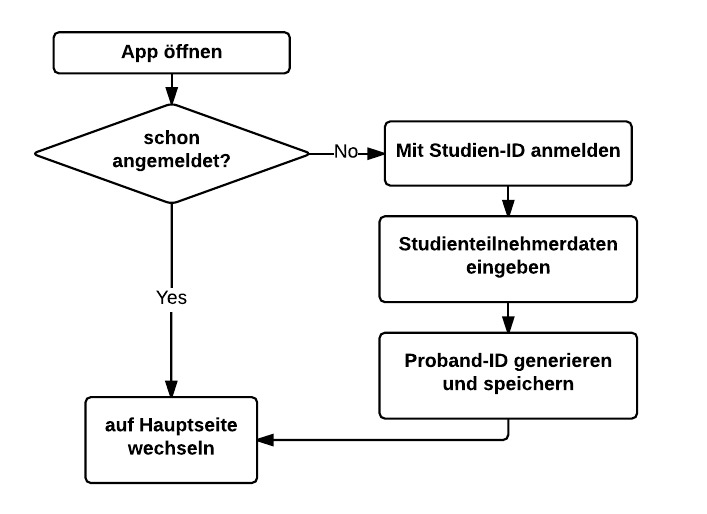
\includegraphics[scale=1]{AppAnmelden.jpeg}
                    \caption{Anmelden der \gls{Proband}en}
                \end{figure}


            \item \textbf{/F80/Beantworten eines Fragebogens}

                \par \textbf{Ziel: }Sammeln der Antworten auf den Fragebogen
                \par \textbf{Vorbedingung: }Anmeldung und mindestens ein vorliegender Fragebogen in der App
                \par \textbf{Nachbedingung: }die Antworten werden lokal gespeichert
                \par \textbf{Akteure: }\gls{Proband}
                \par \textbf{Auslösendes Ereignis: }\gls{Proband} erhaltet Notifikation
                \par \textbf{Beschreibung: }
                \par 1. Wenn ein zu beantwortender Fragebogen vorliegt, schickt die App eine Notifikation.
                \par 2. Nachdem der \gls{Proband} sich angemeldet hat, liegt die App auf der Hauptseite mit einer Liste der auszufüllenden Fragebögen. Der \gls{Proband} wählt einen Fragebogen aus und beantwortet alle darauf stehenden Fragen. Im Anschluss klickt der \gls{Proband} auf ``Send'' und die Antworten werden lokal gespeichert.
                \par \textbf{Alternativen: }
                \begin{figure}[ht]
                    % \raggedleft
                    \centering
                    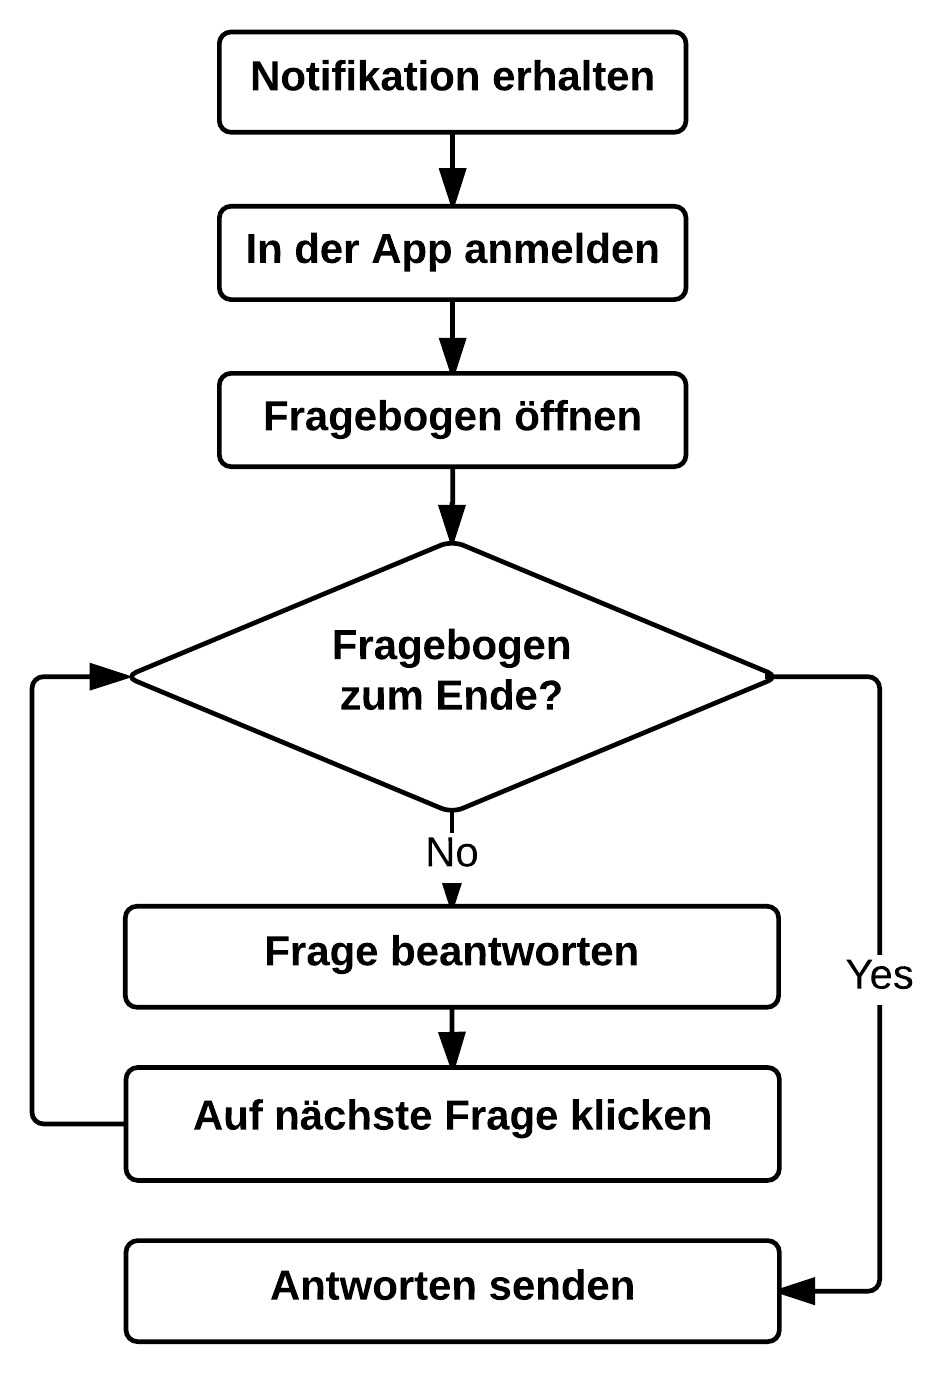
\includegraphics[scale=0.5]{AppAntworten.jpeg}
                    \caption{Antworten eines Fragebogens}
                \end{figure}


            \item \textbf{/F90/Versenden der Antworten eines Fragebogens}

            \par \textbf{Ziel: }Versenden der Antworten an den Server
            \par \textbf{Vorbedingung: }die Antworten werden lokal gespeichert
            \par \textbf{Nachbedingung (Erfolg): }die Antworten werden auf dem Server gespeichert
            \par \textbf{Nachbedingung (Fehlschlag): }die Antworten werden nicht auf dem Server gespeichert
            \par \textbf{Akteure: }App und Server
            \par \textbf{Auslösendes Ereignis: }die Netzwerkverbindung ist verfügbar und es gibt lokal gespeicherte Antworten
            \par \textbf{Beschreibung: }
            \par Wenn die Netzwerkverbindung vorhanden ist, schickt die App die verfügbaren Antworten an den Server und die Antworten werden auf dem Server gespeichert.
            \par \textbf{Alternativen: }
            \begin{figure}[ht]
                % \raggedleft
                \centering
                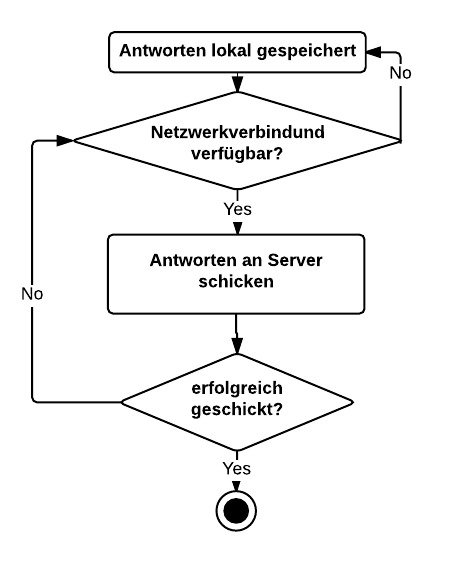
\includegraphics[scale=1.2]{AppVersenden.jpeg}
                \caption{Versenden der Antworten eines Fragebogens}
            \end{figure}

        \end{itemize}

    \chapter{Produktdaten}
        \section{\gls{Studienleiter}daten}
            \begin{itemize}
                \item \textbf{/D10/} Über einen \gls{Studienleiter} sind folgende Daten zu speichern:
                    \par Name (Anrede, Titel, Vorname, Nachname), Mailadresse (als Kontonummer im System)

                \item \textbf{/D20/} Macht ein \gls{Studienleiter} Studien, dann sind folgende Daten zu speichern:
                    \par Studie-IDs der zum \gls{Studienleiter} gehörten Studien
            \end{itemize}

        \section{\gls{Proband}daten}
            \begin{itemize}
                \item \textbf{/D30/} Über einen \gls{Proband} sind folgende Daten zu speichern:
                    \par \gls{Proband}-ID, Geburtsdatum, Beruf, Geschlecht, Studie-ID der daran beteiligten Studie
            \end{itemize}

        \section{Studiendaten}
            \begin{itemize}
                \item \textbf{/D50/} Über eine Studie sind folgende Daten zu speichern:
                    \par Studie-ID, Studiename, Anfangs- und Endedatum, Mailadresse des \gls{Studienleiter}s

                \item \textbf{/D60/} Hat eine Studie \gls{Proband}en, dann sind folgende Daten zu speichern:
                    \par \gls{Proband}-IDs

                \item \textbf{/D70/} Hat eine Studie Fragebogen, dann sind folgende Daten zu speichern:
                    \par Fragebogennummer des Fragebogens
            \end{itemize}

        \section{Fragebogendaten}
            \begin{itemize}
                \item \textbf{/D80/} Über einen Fragebogen sind folgende Daten zu speichern:
                \par Fragebogennummer, Name, Studie-ID der zugehörigen Studie

                \item \textbf{/D90/} Wird ein Fragebogen in der Studie erscheinen, dann sind folgende Daten zu speichern:
                \par Erscheinungsereignisse, Abgabetermin (immer eine Zeit, z.B. 2 Studen nach der Erscheinung des Fragebogens)

                \item \textbf{/D100/} Wird einen Fragebogen von \gls{Proband}en beantwortet, dann sind folgende Daten zu speichern:
                \par \gls{Proband}-IDs der Antwortgeber, Abgabezeit der Antworten, Erscheinungsereignisse, Anzahl der Antworten, Inhalt der Antworten, Ausschöpfungsquote (response rate)
            \end{itemize}

        \section{Fragendaten}
            \begin{itemize}
                \item \textbf{/D110/} Über eine Frage sind folgende Daten zu speichern:
                    \par Fragenummer, Fragetyp, Inhalt der Frage, Fragebogennummer des zugehörigen Fragebogens

                \item \textbf{/D120/} Hat eine Frage Folgefragen, dann sind folgende Daten zu speichern:
                    \par Fragenummern der Folgefragen, Bedingung der Folgefragen (Falls man die bestimmte Optionen der Frage wählt, wird die Folgefragen erscheinen.)
            \end{itemize}

   \chapter{Nichtfunktionale Anforderungen}
        \begin{itemize}
            \item \textbf{/NF10/} Reaktionszeit
                \par Die App darf nicht mehr als 2 Sekunden Reaktionszeit haben und die Ladezeit muss unter 5 Sekunden liegen.

            \item \textbf{/NF20/} Leicht lokalisierbar
                \par Die UI-Sprache wird nicht in dem Programm fix codiert. Neue Sprache-Packe sind leicht zu implementieren.

            \item \textbf{/NF30/} Größe der App
                \par Die App darf nicht mehr als 30 Mb auf dem Handy benötigen.

            \item \textbf{/NF40/} Verschlüsselung der Daten
                \par Die Daten-Tausche müssen verschlüsselt sein. Kein Datum ist vom Dritter erreichbar.
                
            \item \textbf{/NF50/} Länge der Passwörter
                \par Passwörter müssen mindestens 6-stellig sein.
                
            \item \textbf{/NF60/} Probandanzahl
            \par Es müssen maximal 1000 Versuchen mit je maximal 1000 Probanden verwaltet werden können.
        \end{itemize}

    % \chapter{Benutzungsoberfläche}
    %     \subsection{\gls{Web-Interface}}
    %         \begin{figure}[ht]
    %             \centering
    %             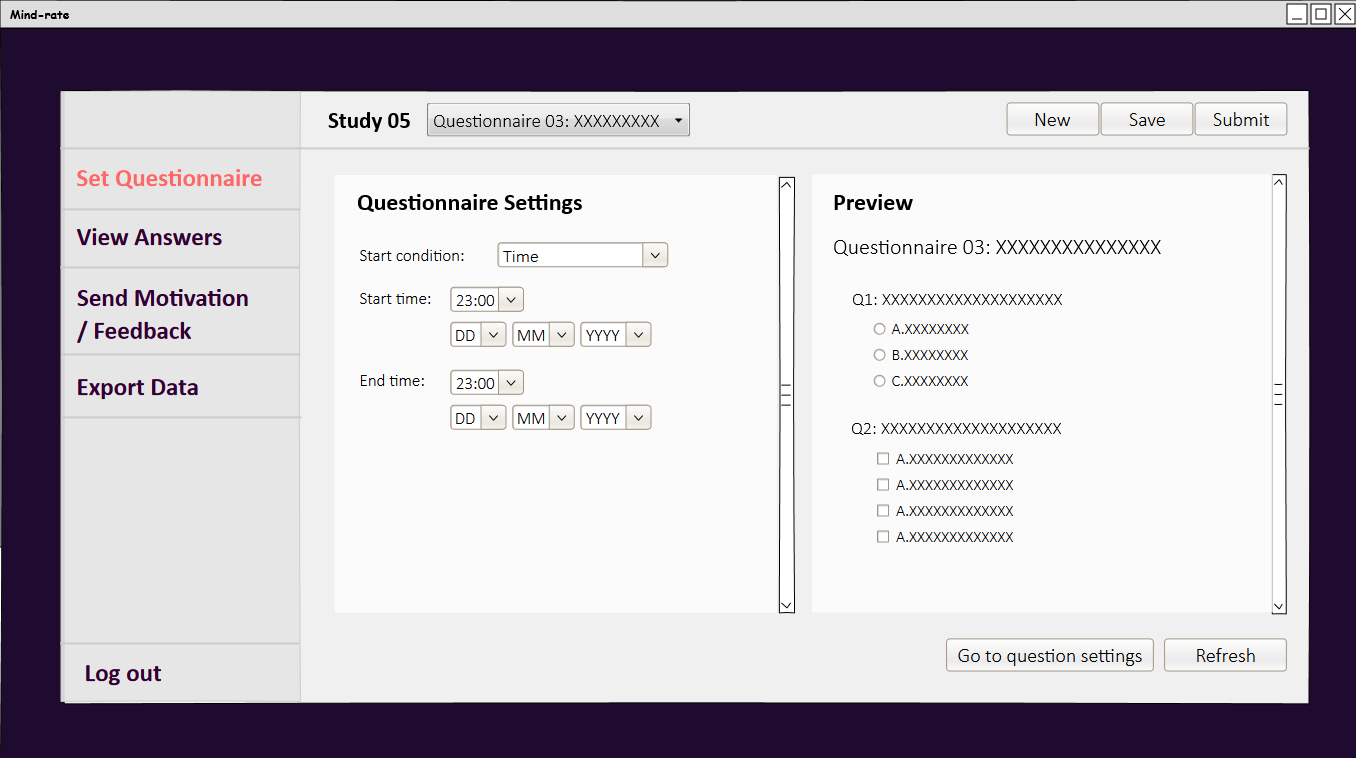
\includegraphics[scale = 0.25]{web_set1.png}
    %             \caption{GUI Entwurf - Questionnaire Settings}
    %         \end{figure}

	   %      \begin{figure}[ht]
	   %      	\centering
	   %      	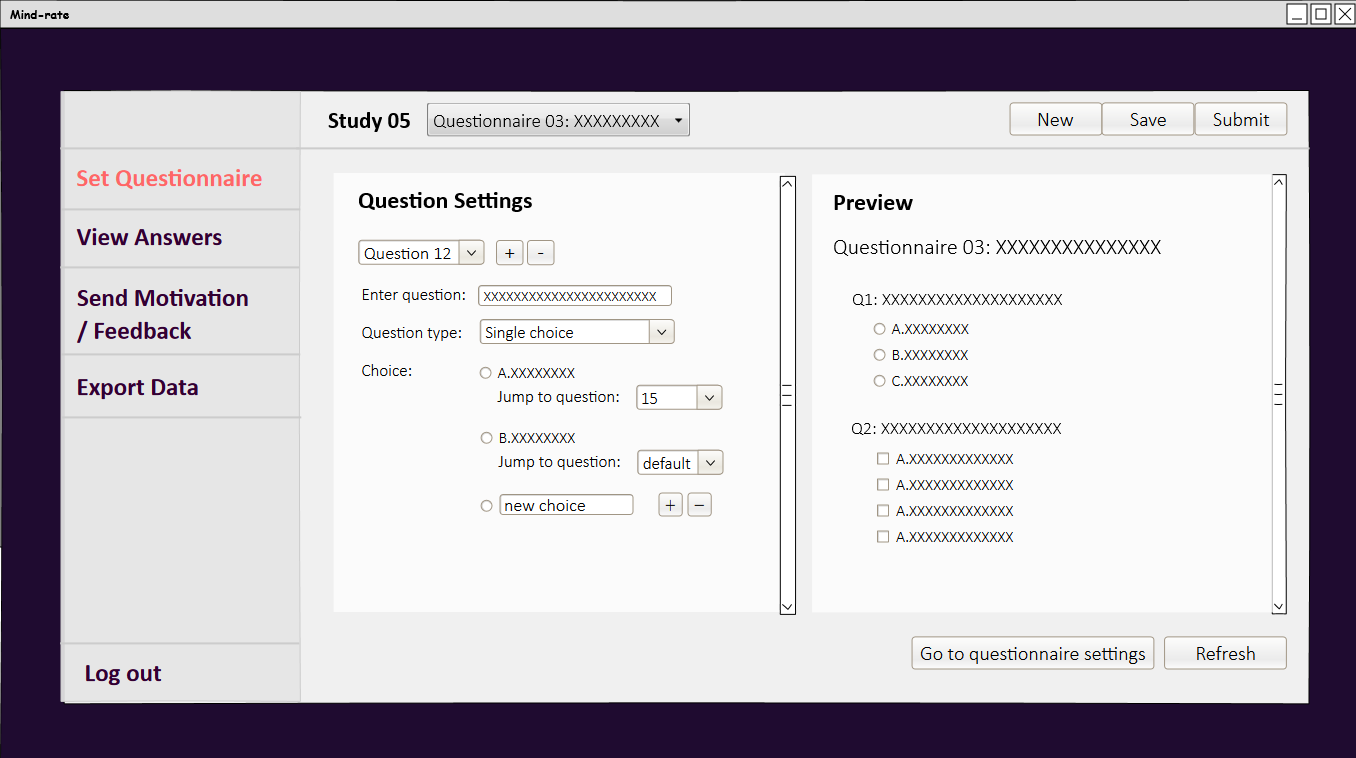
\includegraphics[scale = 0.25]{web_set2.png}
	   %      	\caption{GUI Entwurf - Question Settings}
	   %      \end{figure}

    %         \begin{figure}[ht]
    %             \centering
    %             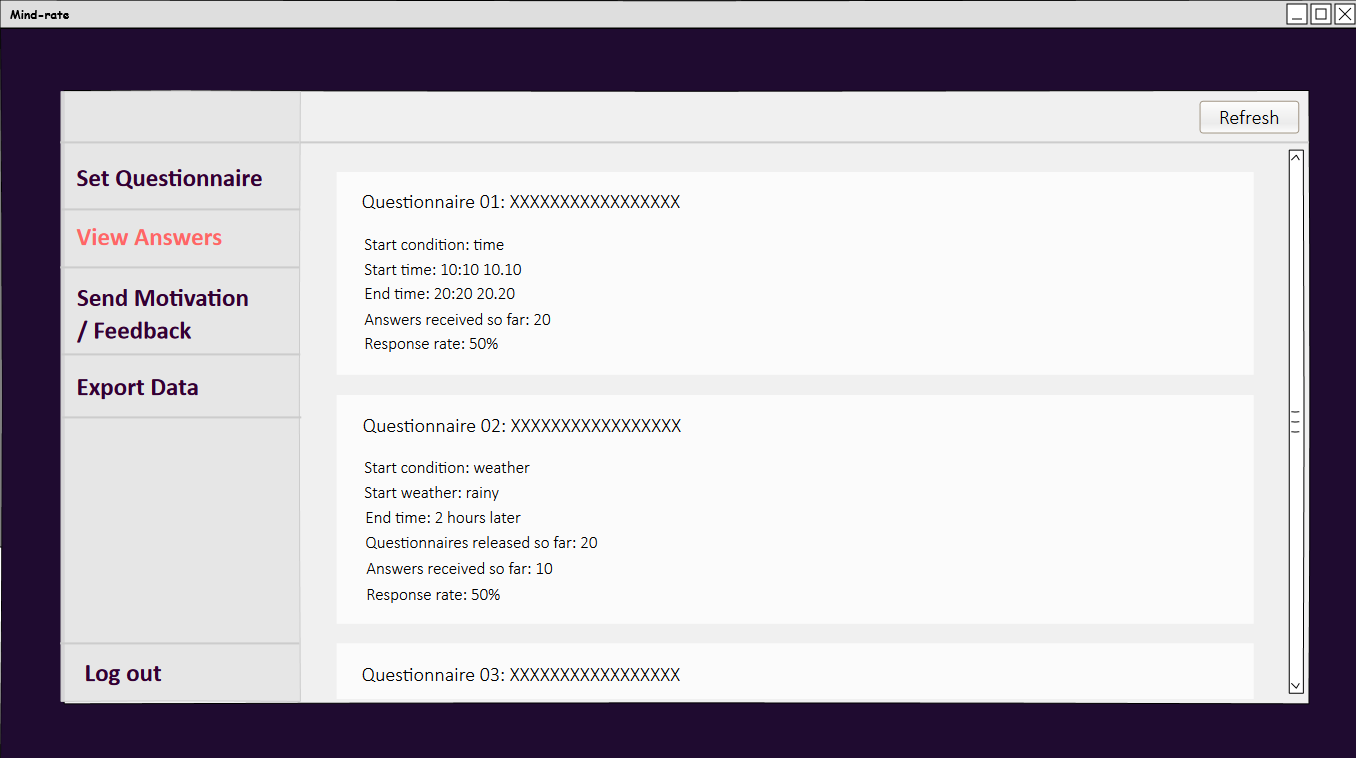
\includegraphics[scale = 0.25]{web_answer.png}
    %             \caption{GUI Entwurf - View Answer}
    %         \end{figure}

    %     \newpage
    %     \subsection{\gls{Android-App}}
    %         \vspace*{2cm}

    %         \begin{figure}[ht]
    %         	\centering
    %         	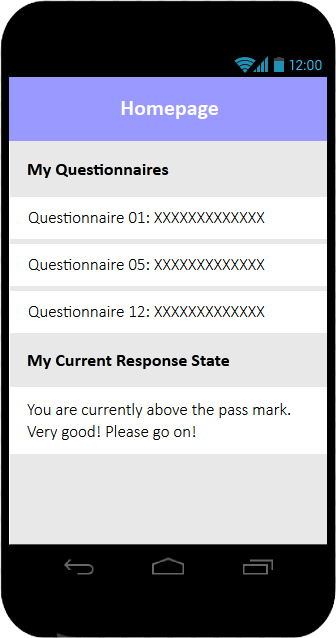
\includegraphics[scale = 0.3]{android_home.jpg}
    %         	\caption{GUI Entwurf - Homepage}
    %         \end{figure}

    %         \vspace*{1cm}
    %         \begin{figure}[ht]
    %             \centering
    %             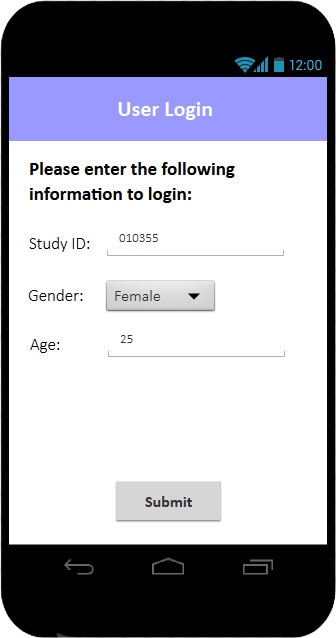
\includegraphics[scale = 0.3]{android_login.jpg}
    %             \caption{GUI Entwurf - Login}
    %         \end{figure}

    %         \vspace*{1cm}
    %         \begin{figure}[ht]
    %             \centering
    %             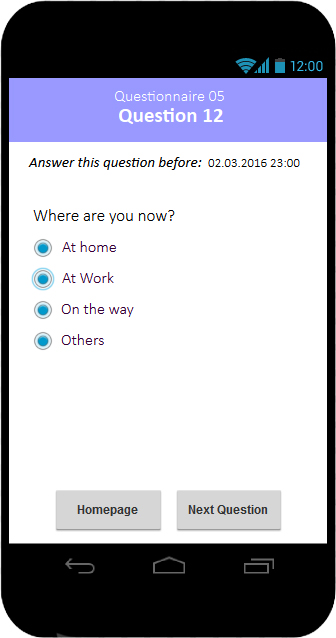
\includegraphics[scale = 0.3]{android_answer.jpg}
    %             \caption{GUI Entwurf - Answer Question}
    %         \end{figure}	

    \chapter{Globale Testfälle}

        Folgende Funktionssequenzen sind zu \"uberpr\"ufen:

        \section{\gls{Web-Interface}}

            \begin{itemize}
                \item \textbf{/TF10/ Registrieren des \gls{Studienleiter}s}
                    \begin{enumerate}
                        \item \par \textbf{Stand: }Offene Homepage des \gls{Web-Interface}
                            \par \textbf{Aktion: }Benutzer klickt auf den Button ``Sign up''
                            \par \textbf{Reaktion: }Der browser wird zu der Registrieren-Seite umgeleitet
                        \item \par \textbf{Stand: }Benutzer ist in der Registrieren-Seite
                             \par \textbf{Aktion: }Benutzer gibt eine Email-Adresse und ein Passwort wird ein
                             \par \textbf{Reaktion: }Eine Bestätigungsmail wird nach dieser Email-Adresse geschenkt
                   \end{enumerate}

                    \item \textbf{/TF20/ Anmelden des \gls{Studienleiter}s}
                        \begin{enumerate}
                            \item \par \textbf{Stand: }Offene Homepage des \gls{Web-Interface}
                                \par \textbf{Aktion: }Registrierte Email-Adresse und Passwort eingeben, und auf “Sign in” klicken
                                \par \textbf{Reaktion: }Erfolgreich eingeloggt. Der browser wird zum Dashboard umgeleitet.
                        \end{enumerate}

                \item \textbf{/TF30/ Vergessenes Passwort neu setzen}
                    \begin{enumerate}
                        \item \par \textbf{Stand: }Offene Homepage des \gls{Web-Interface}
                              \par \textbf{Aktion: }Auf ``Forgot Passwort'' klicken
                              \par \textbf{Reaktion: }Der browser wird zu der Email-Adresse-Eingeben-Seite umgeleitet
                        \item \par \textbf{Stand: }Offene Email-Adresse-Eingeben-Seite
                              \par \textbf{Aktion: }Email-Adresse eingeben, und auf ``Send email'' klicken
                              \par \textbf{Reaktion: }Ein Mail mit einem neuen zufällig generierten Passwort wird zu dieser Email-Adresse geschenkt
                    \end{enumerate}

                \item \textbf{/TF40/ Verwaltung des Fragebogens}
                    \begin{enumerate}
                        \item \par \textbf{Stand: }Kein Fragebogen vorhanden
                              \par \textbf{Aktion: }Der \gls{Studienleiter} klickt auf ``Go to question settings'' Button
                              \par \textbf{Reaktion: }Ein Dialogfeld ``Kein Fragebogen vorhanden.'' erscheint
                        \item \par \textbf{Stand: } Kein Fragebogen vorhanden
                              \par \textbf{Aktion: }Der \gls{Studienleiter} klickt auf ``save'' Button
                              \par \textbf{Reaktion: }Ein Dialogfeld ``Kein Fragebogen vorhanden.'' erscheint
                        \item \par \textbf{Stand: }Kein Fragebogen vorhanden
                              \par \textbf{Aktion: }Der \gls{Studienleiter} klickt auf ``submit'' Button
                              \par \textbf{Reaktion: }Ein Dialogfeld ``Kein Fragebogen vorhanden.'' erscheint
                        \item \par \textbf{Stand: }Kein Fragebogen vorhanden
                              \par \textbf{Aktion: }Der \gls{Studienleiter} klickt auf ``new'' Button
                              \par \textbf{Reaktion: }Der \gls{Studienleiter} kann der Name eines Fragebogens eingeben und dieser Fragebogen wird erstellt
                        \item \par \textbf{Stand: }Ein Fragebogen ausgewählt
                              \par \textbf{Aktion: }Der \gls{Studienleiter} klickt auf ``Go to question settings'' Button
                              \par \textbf{Reaktion: }Der Browser wechselt zur Webseite für die Verwaltung der Fragen
                        \item \par \textbf{Stand: }Ein Fragebogen ausgewählt und eingestellt
                              \par \textbf{Aktion: }Der \gls{Studienleiter} klickt auf ``save'' Button
                              \par \textbf{Reaktion: }Ein Dialogfeld ``Fragebogen wird gespeichert'' erscheint
                        \item \par \textbf{Stand: }Ein Fragebogen gespeichert
                              \par \textbf{Aktion: }Der \gls{Studienleiter} klickt auf ``Refresh'' Button
                              \par \textbf{Reaktion: }Die Voransicht des Fragebogens erscheint
                        \item \par \textbf{Stand: }Alle Einstellung fertig aber keine Frage haben
                              \par \textbf{Aktion: }Der \gls{Studienleiter} klickt auf ``submit'' Button
                              \par \textbf{Reaktion: }Ein Dialogfeld ``Bitte mind. eine Frage erstellen'' erscheint
                        \item \par \textbf{Stand: }Alle Einstellung fertig und Frage vorhanden
                              \par \textbf{Aktion: }Der \gls{Studienleiter} klickt auf ``submit'' Button
                              \par \textbf{Reaktion: }Ein Dialogfeld ``Fragebogen wird hochgeladen'' erscheint
                    \end{enumerate}

                \item \textbf{/TF50/ Verwaltung der Fragen}
                        \begin{enumerate}
                        \item \par \textbf{Stand: } Webseite für die Verwaltung der Fragen ist geladen
                              \par \textbf{Aktion: } Der \gls{Studienleiter} klickt auf ``+'' Button, der links neben den Fragenliste liegt
                              \par \textbf{Reaktion: } Eine neue Frage wird in die Fragenliste hinzugefügt

                        \item \par \textbf{Stand: } Webseite für die Verwaltung der Fragen ist geladen und eine Frage von der Frageliste ausgewählt
                              \par \textbf{Aktion: }  Der \gls{Studienleiter} klickt auf ``-'' Button, der links neben den Fragenliste liegt
                              \par \textbf{Reaktion: } die ausgewählte Frage wird in die Fragenliste gelöscht

                        \item \par \textbf{Stand: } Eine Frage von der Frageliste ausgewählt
                              \par \textbf{Aktion: } Der \gls{Studienleiter} klickt auf ``Question type'' Combobox
                              \par \textbf{Reaktion: } Er kann eine Fragenart auswählen

                        \item \par \textbf{Stand: }  Eine Frage von der Frageliste ausgewählt
                              \par \textbf{Aktion: } Der \gls{Studienleiter} klickt auf ``+'' Button, der rechts neben das Textfeld ``new choice'' liegt
                              \par \textbf{Reaktion: } Eine neue Option für die Antwort erstellt

                        \item \par \textbf{Stand: } Eine Frage hat Optionen
                              \par \textbf{Aktion: } Der \gls{Studienleiter} klickt auf der Fragenliste, die unten eine Option der Frage liegt
                              \par \textbf{Reaktion: }Der \gls{Studienleiter} kann eine vorhandene Frage auswählen

                        \item \par \textbf{Stand: }  Verwaltung der Fragen fertig
                              \par \textbf{Aktion: } Der \gls{Studienleiter} klickt auf ``Refresh'' Button
                              \par \textbf{Reaktion: } Die Voransicht des Fragebogens erneuet

                        \item \par \textbf{Stand: } Verwaltung der Fragen fertig
                              \par \textbf{Aktion: } Der \gls{Studienleiter} klickt auf ``Go to questionnaire settings'' Button
                              \par \textbf{Reaktion: } Der Browser wechselt zur Webseite für die Verwaltung des Fragebogens

                    \end{enumerate}


                \item \textbf{/TF60/ Antwortsstatus besichtigen}
                    \begin{enumerate}
                        \item \par \textbf{Stand: } Der \gls{Studienleiter} ist noch nicht angemeldet.
                              \par \textbf{Aktion: } Der \gls{Studienleiter} klickt den Button ``View Answers''
                              \par \textbf{Reaktion: } Es wrid zur Anmeldungsseite wechseln.

                        \item \par \textbf{Stand: } Der \gls{Studienleiter} ist angemeldet.
                              \par \textbf{Aktion: } Der \gls{Studienleiter} klickt den Button ``View Answers''
                              \par \textbf{Reaktion: } Der \gls{Studienleiter} kann die \"ubersicht von allen Antwort sehen.

                        \item \par \textbf{Stand: } Der \gls{Studienleiter} bleibt in der Seite ``View Answers''
                              \par \textbf{Aktion: } Der \gls{Studienleiter} klickt den Button ``Refresh''
                              \par \textbf{Reaktion: } Die neue \"ubersicht von allen Antwort wird gezeigt.

                        \item \par \textbf{Stand: } Der \gls{Studienleiter} bleibt in der Seite ``View Answers''
                              \par \textbf{Aktion: } Der \gls{Studienleiter} gibt einige Bedingungen ein und klickt er den Button ``Confirm''
                              \par \textbf{Reaktion: } Die Antwort wird gefiltert. Die \"ubersicht von Antwort der \gls{Proband}en, die alle eingegebene Bedingungen erf\"ullen, wird geladen.\"ubersicht
                    \end{enumerate}
                    % \begin{itemize}
                    %     \item Durch Klicken von Button ``View answers'' in der linke Men\"u siehe der \gls{Studienleiter} die \"Ubersicht von allen Antwort des aktuellen Fragebogens. \\
                    %     (Abbildung \ref*{web_ViewAnswer})
                    %     \item Durch Klicken von Button ``Refresh'' wird die neuese \"Ubersicht geladen.
                    %     \item Nach Eingeben von verschiedenene Kriterien wird die \"Ubersicht von Antwort der bestimmten \gls{Proband}en gezeigt.
                    % \end{itemize}

                \item \textbf{/TF65/ Feedback (Motivation) senden}

                    \begin{enumerate}
                        \item \par \textbf{Stand: } Der \gls{Studienleiter} ist noch nicht angemeldet.
                              \par \textbf{Aktion: } Der \gls{Studienleiter} klickt den Button ``Send Motivation / Feedback''
                              \par \textbf{Reaktion: } Es wrid zur Anmeldungsseite wechseln.
                        \item \par \textbf{Stand: } Der \gls{Studienleiter} ist angemeldet.
                              \par \textbf{Aktion: }  Der \gls{Studienleiter} klickt den Button ``Send Motivation / Feedback''
                              \par \textbf{Reaktion: } Der \gls{Studienleiter} wird zur Seite hergeleitet, wo er Motivation / Feedback schreiben und senden kann.
                        \item \par \textbf{Stand: } Der \gls{Studienleiter} bleibt in der Seite ``Send Motivation / Feedback''
                              \par \textbf{Aktion: } Der \gls{Studienleiter} hat die Motivation fertig geschrieben und klickt er den Button ``send''.
                              \par \textbf{Reaktion: } Die Smartphone von \gls{Proband} erh\"alt eine Notifikation. Durch Klicken von dieser Notifikation kann der \gls{Proband} die Motivation sehen.
                        % \item \par \textbf{Stand: }
                        %       \par \textbf{Aktion: }
                        %       \par \textbf{Reaktion: }
                        % \item \par \textbf{Stand: }
                        %       \par \textbf{Aktion: }
                        %       \par \textbf{Reaktion: }
                    \end{enumerate}


                    % \par Durch Klicken von Button ``Send Motivation / Feedback'' sieht der \gls{Studienleiter} die Seite, wo er Motivation und Feedback schreiben und senden kann.
                    % \par Durch Klicken von Button ``send'' wird die geschriebene Motivation zu allen \gls{Proband}en gesandt.
                    % \par Die Smartphone von \gls{Proband} erh\"alt eine Notifikation. Durch Klicken von dieser Notifikation kann der \gls{Proband} die Motivation sehen.

                \item \textbf{/TF70/ Exportieren von Daten}
                \begin{itemize}
                    \item \par \textbf{Stand: }Sein angemeldet
                          \par \textbf{Aktion: }Klicken auf ``Export data''
                          \par \textbf{Reaktion: }Daten sind exportiert
                \end{itemize}


            \end{itemize}


        \vspace*{2cm}
        \section{\gls{Android-App}}

            \begin{itemize}

            \item \textbf{/TF-/ Erstes Anmelden der \gls{Proband}en}
            \begin{enumerate}
                \item \par \textbf{Stand: }Der \gls{Proband} hat sich noch nicht in der App angemeldet
                \par \textbf{Aktion: }Der \gls{Proband} öffnet die App
                \par \textbf{Reaktion: }Die App wechselt auf die ``User Login'' Seite
                \item \par \textbf{Stand: }Die ``User Login'' Seite liegt vor
                \par \textbf{Aktion: }Der \gls{Proband} gibt Studie-ID und die angeforderte Information ein, und klickt den Button ``Submit''
                \par \textbf{Reaktion: }Der \gls{Proband} wird auf die Hauptseite weitergeleitet
            \end{enumerate}

	        \item \textbf{/TF-/ Automatisches Anmelden der \gls{Proband}en}
	        \begin{enumerate}
	        	\item \par \textbf{Stand: }Der \gls{Proband} hat sich schon einmal in der App angemeldet
	        	\par \textbf{Aktion: }Der \gls{Proband} öffnet die App
	        	\par \textbf{Reaktion: }Der \gls{Proband} wird automatisch auf die Hauptseite weitergeleitet
	        \end{enumerate}

	        \item \textbf{/TF-/ Antworten eines Fragebogens}
	        \begin{enumerate}
	        	\item \par \textbf{Stand: }Die Hauptseite der App liegt vor
	        	\par \textbf{Aktion: }Der \gls{Proband} wählt einen Fragebogen aus ``My Questionnaires''
	        	\par \textbf{Reaktion: }Der \gls{Proband} wird auf die erste Frage des gewählten Fragebogens weitergeleitet
	        	\item \par \textbf{Stand: }Der \gls{Proband} ist auf der Seite einer Frage
	        	\par \textbf{Aktion: }Der \gls{Proband} beantwortet die Frage und klickt den Button ``Next Question''
	        	\par \textbf{Reaktion: }Der \gls{Proband} wird auf die nächste Frage des Fragebogens weitergeleitet
	        	\item \par \textbf{Stand: }Der \gls{Proband} ist auf der Seite einer Frage
	        	\par \textbf{Aktion: }Der \gls{Proband} klickt den Button ``Homepage''
	        	\par \textbf{Reaktion: }Der \gls{Proband} wird auf die Hauptseite weitergeleitet und die schon eingegebenen Antworten des Fragebogens werden nicht gespeichert
	        	\item \par \textbf{Stand: }Der \gls{Proband} ist auf der Seite letzter Frage des Fragebogens
	        	\par \textbf{Aktion: }Der \gls{Proband} beantwortet die Frage und klickt den Button ``Submit''
	        	\par \textbf{Reaktion: }Die App zeigt ``You have successfully submitted your answers!'' und wechselt auf die Hauptseite
	        \end{enumerate}

            \end{itemize}

    \chapter{Systemmodelle}

        \section{Szenarien}

        % \"
            \subsection{Szenario 1}
                Ein super psychologischer Expert Prof. Dr. Mata beschliesst, eine Studie nach ESM Methode durchzuf\"uhren. Er \"offnet den browser und die mind-Rate web-Anwendung. Nach Eingeben g\"ultiger Email-Adresse und Passwort gelingt ihm zu registrieren und erh\"alt er dann eine Bestätigungsmail. \\
                Nach Anmeldung setzt Prof. Dr. Mata zun\"achst die Name, ID, Dauer (von wann bis wann) seiner Studie. Er entscheidet sich, die Studie ``Hello World'' mit ID ``9527'' zu nennen und die Studie wird 2 Monate dauern. Dann klickt er den Button ``Set Questionnaire'' und er wird zu die Seite hergeleitet, wo er die auslösende Ereiginisse und G\"ultigkeitszeitbereich eines Fragebogens setzen kann. Daf\"ur setzt er ``everyday 10am'' und ``30 minute''. \\
                Danach klickt Prof. Dr. Mata den Button ``Go to question settings''. Die Seite ``Question setting'' kommt vor. Auf dieser Seite ist Prof. Dr. Mata in der Lage, die Frage einzugeben und Art der Frage auszuw\"ahlen. F\"unf Fragenarten sind verf\"ugbar: ``Single-Choice-Frage'', ``Multiple-Choice-Frage'', ``Skala-mit-Stufen-Frage'', ``Skala-ohne-Stufe-Frage'' und ``Offene Frage''. \\
                Prof. Dr. Mata schreibt die erste Frage ``Where are you?'' and setzt sie als ``Single-Choice-Frage''. Für Antwort stellt er 4 Optionen zu Verf\"ugung: ``Home'', ``Work'', ``Travel'', ``On the way''. Die erste Frage tritt dann rechts auf, wo sich die Preview des Fragebogens befindet. Dann klickt er den Button ``+'', f\"ugt er die zweite Frage ``Where are you heading to?'' hinzu und setzt er diese Frage als ``Offene Frage''. Danach schreibt er die dritte Frage ``How do you feel?'' und beschliesst, diese Frage als ``Skala-mit-Stufen-Frage'' zu definieren. Deswegen erstellt er 5 Stufen: ``really bad'', ``bad'', ``Ok'', ``good'', ``very good''. \\
                Pl\"otzlich findet Prof. Dr. Mata, dass die Dauer der Studie, 2 Monate,  zu lang ist. Daher klickt er den Button ``Go to questionnaire settings'' und wechselt er zu die Seite ``Questionnaire settings''. Nachdem er die \"Anderung erledigt, druckt er den Button ``Go to question settings'' und wechselt er wieder zu die Seite ``Question setting''. \\
                Prof. Dr. Mata denkt, dass es sinnlos ist, die zweite Frage zu beantworten, falls die Probanden Optionen ``Home'' und ``Work'' f\"ur die erste Frage gew\"ahlt haben. Weswegen wechselt er zu die Seite f\"ur die erste Frage und w\"ahlt er ``3'' f\"ur'``jump to question''-Setzung unter Optionen ``Home'' und ``Work''. \\
                Schliesslich hat Prof. Dr. Mata diesen Fragebogen fertig erstellt. Er klickt dann den Button ``save'' und ``submit''. Danach macht er Pause und habt er vor, neuen Fragebogen zu erstellen...\\
            \subsection{Szenario 2}
            \subsection{Szenario 3}

        \newpage
        \section{Anwendungsfalldiagramm}
            \vspace*{2cm}
            \begin{figure}[htbp]
                \centering
                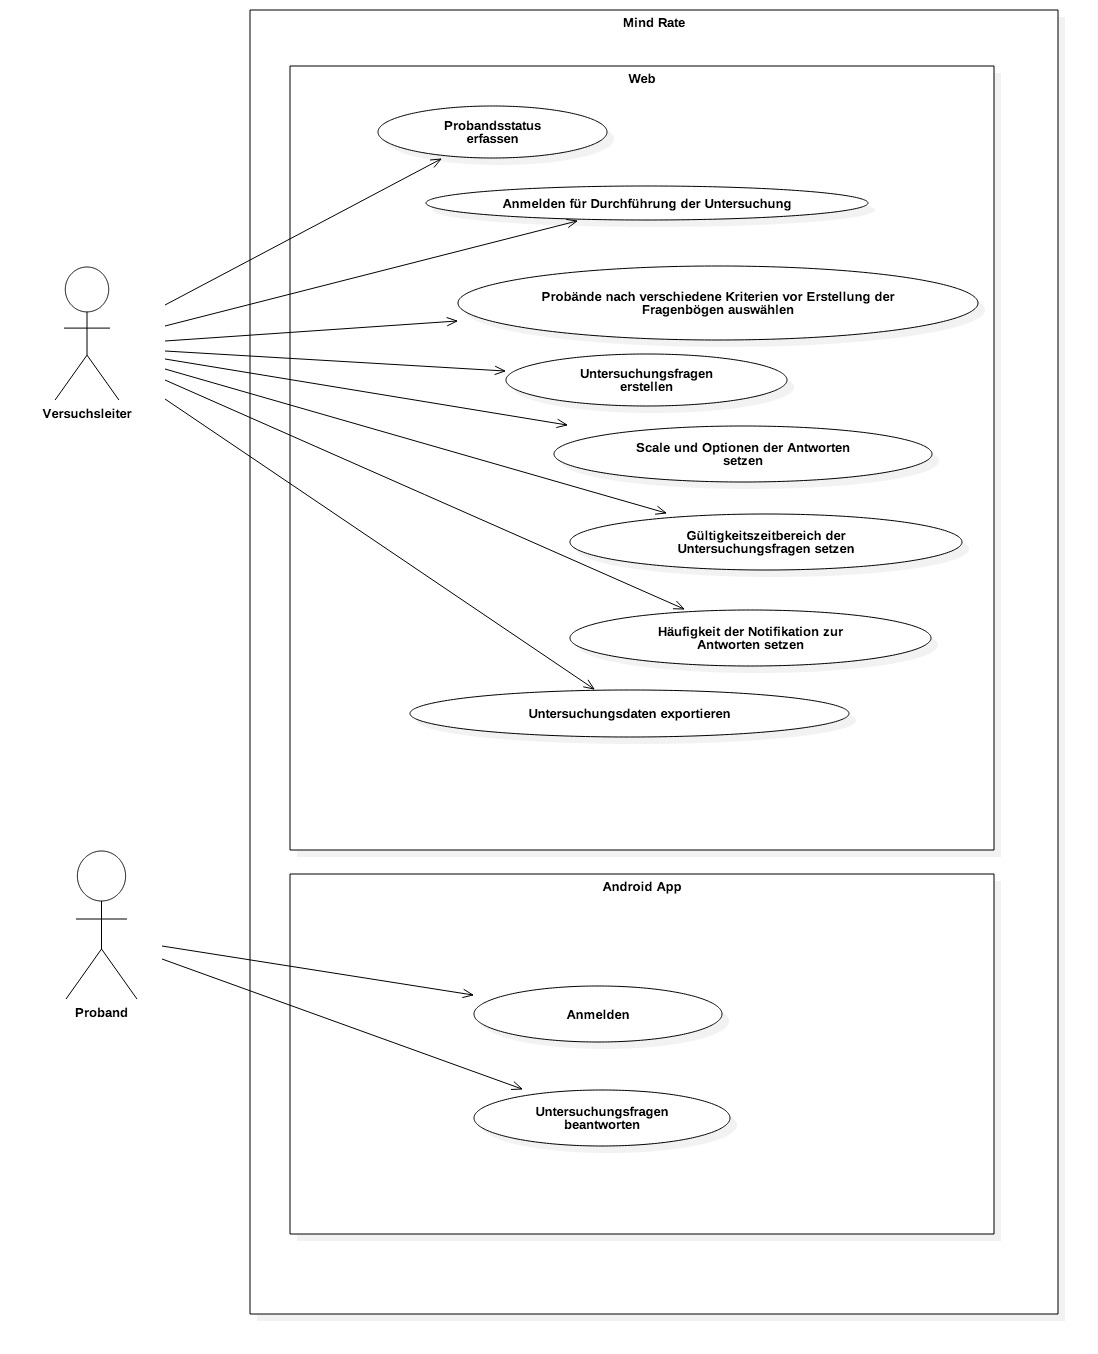
\includegraphics[scale = 0.4]{UseCaseDiagram1.jpg}
                \caption{Anwendungsfalldiagramm}
            \end{figure}

        \newpage
        \section{Benutzerschnittstelle}

            \vspace*{1cm}
            \subsection{\gls{Web-Interface}}
                \vspace*{1.5cm}
                \begin{figure}[ht]
                    \centering
                    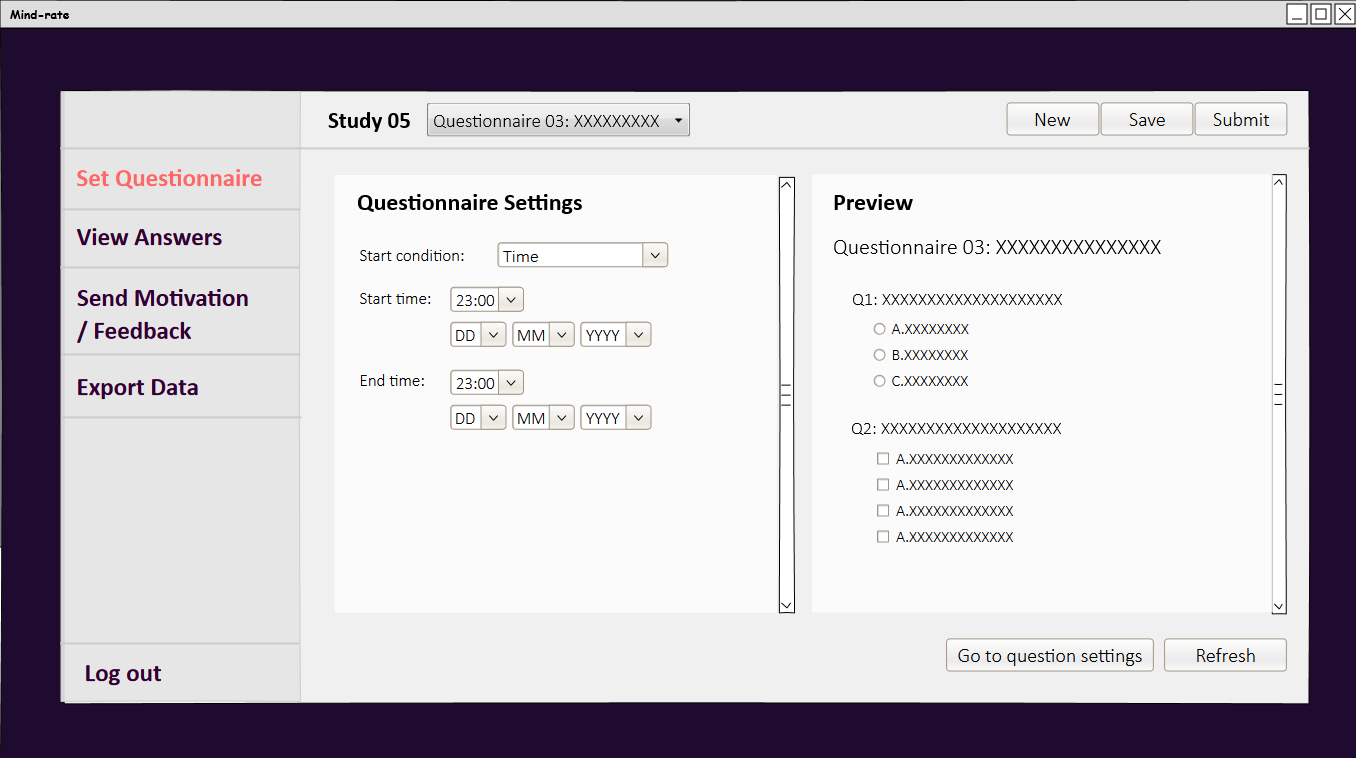
\includegraphics[scale = 0.25]{web_set1.png}
                    \caption{GUI Entwurf - Questionnaire Settings}
                \end{figure}

                \begin{figure}[ht]
                    \centering
                    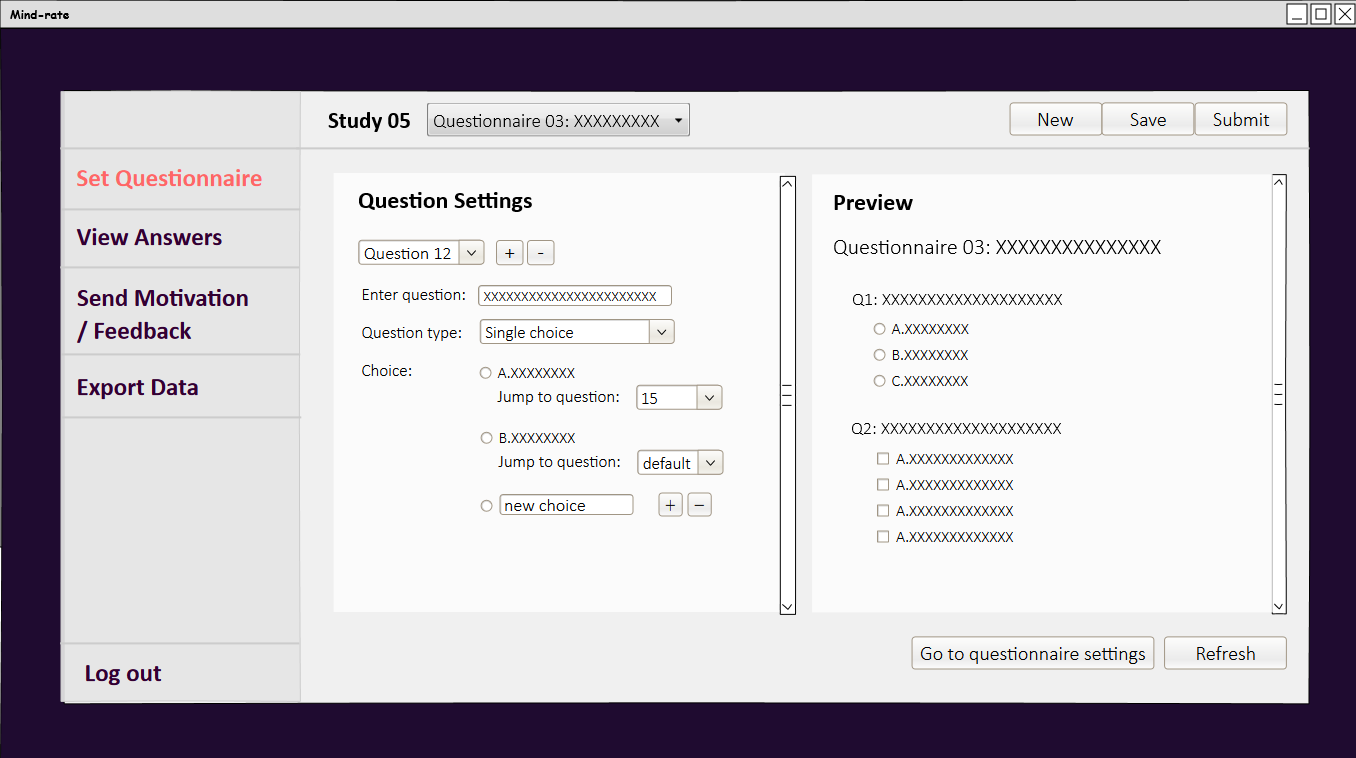
\includegraphics[scale = 0.25]{web_set2.png}
                    \caption{GUI Entwurf - Question Settings}
                \end{figure}

                \begin{figure}[ht]
                    \centering
                    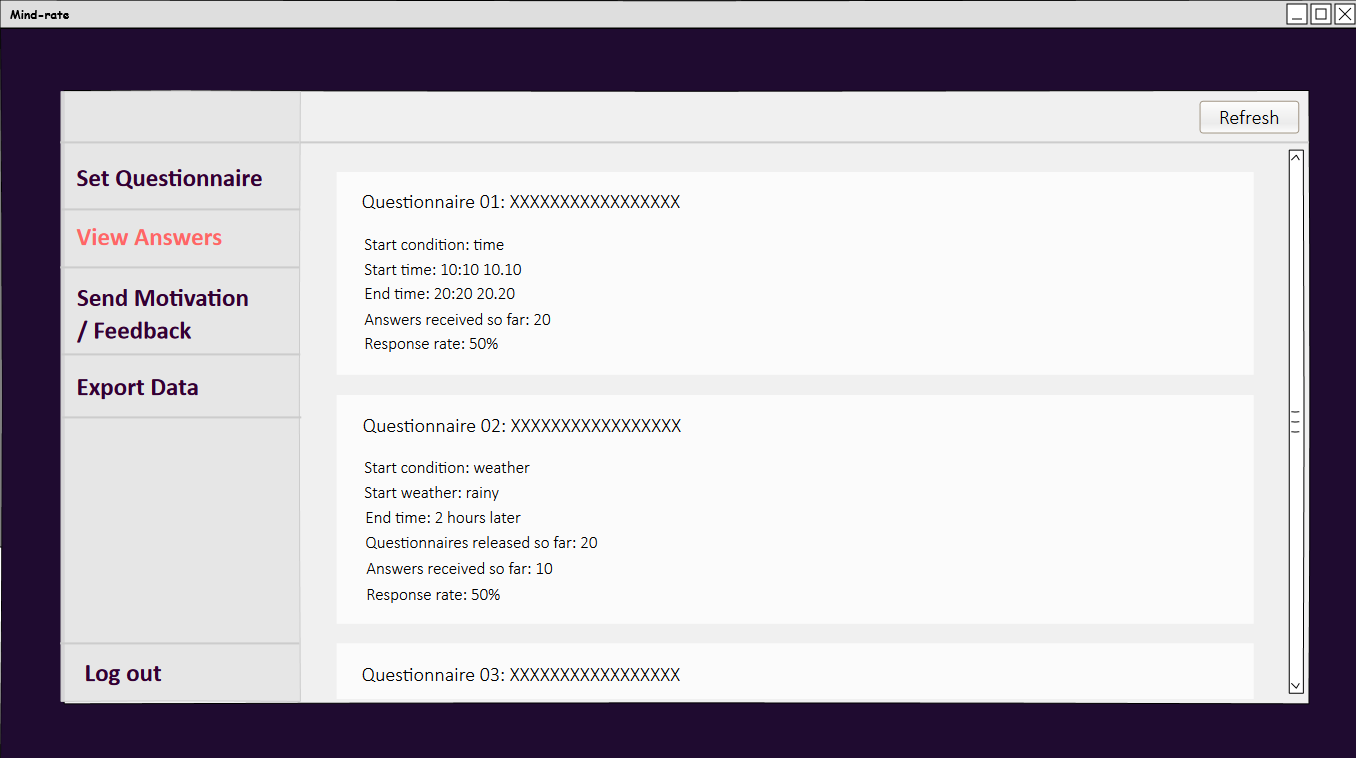
\includegraphics[scale = 0.25]{web_answer.png}
                    \caption{GUI Entwurf - View Answer}
                \end{figure}

            \newpage
            \subsection{App}
                \vspace*{2cm}

                \begin{figure}[ht]
                    \centering
                    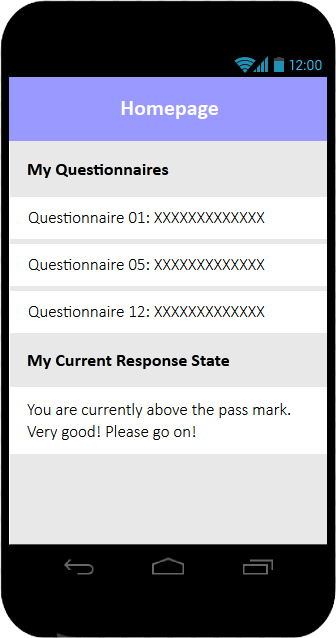
\includegraphics[scale = 0.3]{android_home.jpg}
                    \caption{GUI Entwurf - Homepage}
                \end{figure}

                \vspace*{1cm}
                \begin{figure}[ht]
                    \centering
                    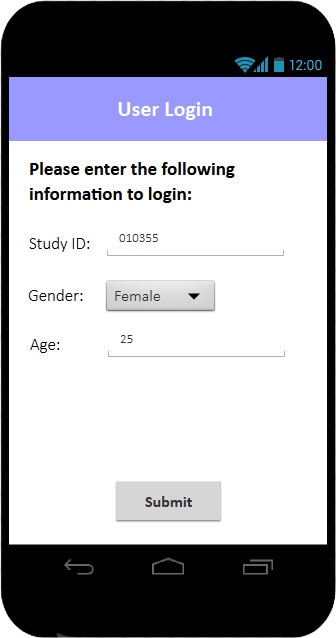
\includegraphics[scale = 0.3]{android_login.jpg}
                    \caption{GUI Entwurf - Login}
                \end{figure}

                \vspace*{1cm}
                \begin{figure}[ht]
                    \centering
                    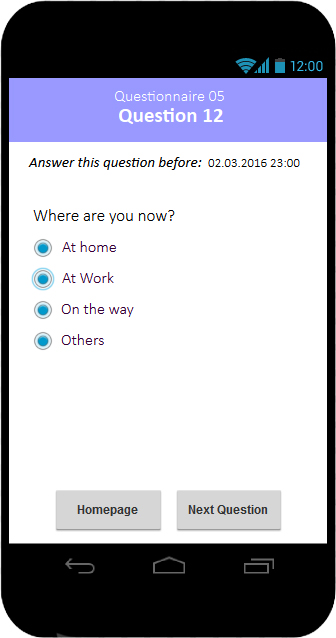
\includegraphics[scale = 0.3]{android_answer.jpg}
                    \caption{GUI Entwurf - Answer Question}
                \end{figure}




%    \chapter{Qualitätsziele}
%        Qualiätsziele: Allgemeine Ziele sind meistens Änderbarkeit und Wartbarkeit.
%        Ziele sollten jedoch grundsätzlich messbar, spezifisch und relevant sein.

    \glsaddall
    \printglossary

    % Abbildungsverzeichnis
    \listoffigures

\end{document}
